\documentclass{article}
\usepackage[total={18cm,21cm},top=2cm, left=2cm]{geometry}
\parindent=0mm
% Otros paquetes -----------------------------------------------------
\usepackage[spanish, es-tabla]{babel} % Idioma español
\usepackage[T1]{fontenc}
\usepackage[utf8]{inputenc} %
\usepackage{mathpazo} % fuente palatino
\usepackage{graphicx,pstricks}
\usepackage{latexsym,amsmath,amssymb,amsfonts,cancel}
\usepackage[shortlabels]{enumitem}
\usepackage[cache=true]{minted}
\usemintedstyle{vs}
\usepackage{multirow}
\usepackage[table,xcdraw,svgnames]{xcolor}
% Referencias - ligas
\usepackage[hyphens]{url}
\usepackage[breaklinks,colorlinks=true,linkcolor=red,
citecolor=red, urlcolor=blue]{hyperref}
% Comandos ------------------------------------------------------------
\newcommand{\sen}{\mathop{\rm sen}\nolimits} % seno
\newcommand{\arcsen}{\mathop{\rm arcsen}\nolimits}
\newcommand{\arcsec}{\mathop{\rm arcsec}\nolimits}
\renewcommand{\arraystretch}{1.5}
\renewcommand{\listtablename}{Tabla}
\setminted{
	linenos,                % Numeración de líneas
	breaklines,             % Romper líneas largas
	breakanywhere,          % Romper en cualquier punto
	tabsize=4,              % Tamaño de tabulación
	fontsize=\small,        % Tamaño de la fuente
	framesep=2mm,           % Espacio entre el código y el marco
	xleftmargin=0.75em,     % Margen izquierdo extra
	xrightmargin=0.75em,    % Margen derecho extra
	bgcolor=lightgray!10,   % Color de fondo muy suave	
	frame=lines,            % Marco superior e inferior
	rulecolor=gray          % Color del marco
}
% ----------------------------------------------------------------------
\begin{document}
	\title{AN\'ALISIS DEL APORTE DE LAS ENERG\'IAS RENOVABLES EN LA GENERACI\'ON EL\'ECTRICA EN COLOMBIA \\		
		{\small \gray {\fontfamily{phv}\selectfont
				Talento Tech\\
				Inteligencia Artificial\\
				Nivel Explorador\\
				}
			}}
		\author{Alba L\'opez \\ Ulises Linares \\ Luis Bertel}
	\date{2025}
\maketitle
\tableofcontents

\newpage

\begin{abstract}
	Este estudio analiza la evolución del aporte de las energías renovables en la generación eléctrica en Colombia entre los años 2010 y 2025, en el contexto de la transición energética y los compromisos nacionales e internacionales de sostenibilidad. Para ello, se utilizó un conjunto de datos con registros mensuales de generación eléctrica por tipo de fuente energética, inicialmente extraído desde la plataforma Kaggle (2010–2022) y posteriormente actualizado mediante técnicas de web scraping hasta el año 2025. La investigación se desarrolló bajo el enfoque del ciclo de vida de proyectos de Machine Learning, e incluyó procesos de limpieza de datos, análisis exploratorio, visualización de tendencias y análisis multidimensional. Las herramientas principales empleadas fueron Python y bibliotecas como Pandas, NumPy, Matplotlib y Seaborn. Los resultados permiten identificar patrones de crecimiento, estacionalidad y participación relativa de las fuentes renovables —como solar, eólica, hidroeléctrica y otras— en la matriz eléctrica colombiana. Este análisis proporciona insumos relevantes para la toma de decisiones en materia de política energética, planificación sectorial y evaluación del avance del país hacia un sistema eléctrico más diversificado y sostenible.
\end{abstract}

%\chapter{LaTeX }
\section{Introducci\'on}

En el contexto actual de transición energética y lucha contra el cambio climático, el análisis de las fuentes utilizadas para la generación de electricidad se ha convertido en una herramienta fundamental para comprender la evolución del sistema energético global. La electricidad es un insumo esencial para prácticamente todas las actividades productivas, sociales y tecnológicas, por lo que su disponibilidad, accesibilidad y sostenibilidad resultan determinantes para el desarrollo económico y el bienestar social.\\

Los sistemas eléctricos están experimentando una transformación profunda impulsada por el avance tecnológico, la creciente penetración de energías renovables, las preocupaciones ambientales y los compromisos internacionales de descarbonización. En este escenario, evaluar la participación relativa de las distintas fuentes de generación —como las tecnologías renovables (hidroeléctrica, solar, eólica, geotérmica), la energía nuclear y los combustibles fósiles (carbón, gas natural, petróleo)— permite no solo entender el comportamiento histórico del sector, sino también anticipar escenarios futuros y sus implicancias a nivel ambiental y económico.\\

Desde una perspectiva ambiental, el tipo de fuente energética utilizada en la generación eléctrica determina en gran medida el volumen de emisiones de gases de efecto invernadero (GEI), así como otros impactos relacionados con el uso del agua, el suelo y la biodiversidad. Por ello, el análisis de la matriz de generación resulta clave para monitorear el progreso hacia metas climáticas y para identificar oportunidades de mejora en términos de eficiencia y sostenibilidad.\\

Desde el punto de vista económico, la diversificación de fuentes y la integración de tecnologías limpias pueden contribuir a reducir la vulnerabilidad frente a fluctuaciones de precios en los mercados energéticos internacionales, mejorar la seguridad energética y estimular la innovación y el desarrollo de nuevas cadenas de valor. Además, una planificación energética basada en datos empíricos permite a los gobiernos y organismos reguladores diseñar políticas públicas más eficaces, promover inversiones sostenibles y garantizar el acceso equitativo a servicios energéticos modernos.\\

En este sentido, el estudio sistemático de los datos sobre generación eléctrica clasificados por tipo de fuente constituye una base sólida para la toma de decisiones informadas, el diseño de políticas integradas y la construcción de sistemas eléctricos más resilientes, sostenibles y socialmente inclusivos.\\

\subsection{Contexto}

Colombia se encuentra en una etapa clave de transformación de su matriz energética, impulsada por la necesidad de diversificar las fuentes de generación eléctrica, reducir la dependencia de recursos hidroeléctricos y fósiles, y avanzar hacia un sistema energético más sostenible y resiliente frente al cambio climático. Históricamente, el país ha contado con una alta participación de la generación hidroeléctrica —superior al 60 \% en varios años—, lo cual ha permitido mantener una baja intensidad de emisiones de carbono en el sector eléctrico en comparación con otras economías de América Latina y el mundo. No obstante, esta dependencia ha expuesto al sistema a riesgos asociados con la variabilidad climática, especialmente durante los períodos de sequía causados por fenómenos como El Niño, que comprometen la estabilidad del suministro energético.\\

Con el objetivo de diversificar su matriz energética y fortalecer su resiliencia, Colombia ha establecido un marco normativo robusto para la promoción de las fuentes no convencionales de energía renovable (FNCER), particularmente las tecnologías solar fotovoltaica y eólica. La Ley 1715 de 2014, junto con desarrollos posteriores como la Ley 2099 de 2021 y las subastas de contratos de largo plazo organizadas por el Ministerio de Minas y Energía, han creado condiciones favorables para la inversión en este tipo de tecnologías. En línea con sus compromisos internacionales, como el Acuerdo de París y su Contribución Determinada a Nivel Nacional (NDC), el país se ha trazado metas ambiciosas para aumentar la participación de energías renovables en su matriz y reducir las emisiones del sector energético.\\

A pesar de estos avances, el desarrollo e integración de las FNCER enfrenta diversos desafíos técnicos, económicos y sociales. Entre ellos se destacan la necesidad de fortalecer la infraestructura de transmisión, adaptar la regulación del mercado eléctrico para facilitar la participación de fuentes intermitentes, resolver aspectos relacionados con la consulta previa en territorios de comunidades étnicas y garantizar la estabilidad financiera de los proyectos a largo plazo. Estos desafíos requieren una planificación energética integral, basada en evidencia empírica y en análisis comparativos que permitan identificar tendencias, oportunidades y barreras.\\

En este contexto, el presente análisis se basa en un conjunto de datos proporcionado por la Agencia Internacional de Energía (AIE), que reúne información mensual sobre la generación eléctrica de múltiples países —incluido Colombia— entre 2010 y 2025. El dataset está estructurado por año, mes, tipo de fuente energética y volumen de generación expresado en gigavatios-hora (GWh). Esta información permite cuantificar y caracterizar la evolución del aporte de las energías renovables a la generación eléctrica nacional, así como comparar el desempeño colombiano con el de otras naciones en la región y el mundo.\\

El análisis de esta información no solo proporciona una visión detallada del proceso de transición energética en Colombia, sino que también contribuye a la formulación de políticas públicas, al diseño de estrategias de inversión y a la promoción de un sistema eléctrico más eficiente, sostenible e inclusivo.\\

\subsection{Definici\'on del problema}

\subsubsection{Objetivo esp\'ecifico}
Analizar la evolución y el aporte de las fuentes de energía renovable en la generación eléctrica en Colombia entre los años 2010 y 2025, con base en datos estadísticos comparativos, a fin de identificar tendencias, avances y desafíos en el marco de la transición energética del país.

\subsubsection{Objetivos esp\'ecificos}

\begin{itemize}
	\item Caracterizar la participación de las diferentes fuentes renovables (solar, eólica, hidroeléctrica, geotérmica y otras) en la matriz de generación eléctrica de Colombia durante el período 2010–2025.
	\item Identificar los principales desafíos y oportunidades asociados a la integración de fuentes renovables en el sistema eléctrico colombiano, en relación con factores técnicos, regulatorios y ambientales.
\end{itemize}


\subsection{preguntas orientadora}

¿Cómo ha evolucionado el aporte de las energías renovables en la generación eléctrica en Colombia entre 2014 y 2025, y qué factores explican su desempeño?


\section{Materiales y métodos}

\subsection{Enfoque metodológico}

Este estudio se enmarca dentro del ciclo de vida de un proyecto de Machine Learning, específicamente en las etapas de adquisición de datos, limpieza, análisis exploratorio, visualización y análisis multidimensional. Aunque no se realiza modelado predictivo, se adoptan herramientas y metodologías propias de la ciencia de datos para estructurar un análisis riguroso, reproducible y orientado a la extracción de conocimiento a partir de datos energéticos. El enfoque se limita exclusivamente al caso de Colombia.

\subsection{Conjunto de datos}

El análisis se basa en un conjunto de datos inicialmente obtenido desde el portal Kaggle, el cual contiene información mensual de generación eléctrica clasificada por tipo de fuente energética, país, año y mes, expresada en gigavatios-hora (GWh). Esta base cubre el período comprendido entre 2010 y 2022. Para extender el alcance temporal hasta 2025, se aplicaron técnicas de web scraping sobre fuentes oficiales y sitios especializados, lo que permitió actualizar el conjunto de datos con los registros más recientes disponibles.\\

El dataset final fue consolidado y almacenado en formato CSV, lo cual facilitó su manipulación y análisis mediante herramientas de programación. Se realizó una curaduría manual y automatizada para garantizar la coherencia, completitud y calidad de los datos utilizados.\\

El conjunto de datos utilizado contiene registros mensuales de generación eléctrica para distintos países, incluyendo Colombia, y presenta la siguiente estructura de variables en la tabla \ref{table:tab1}:

\begin{table}[h!]
	\begin{tabular}{|l|p{14cm}|}
		\hline
		\textbf{Variable}  & \textbf{Descripción}                                                                                                    \\ \hline
		COUNTRY            & Nombre del país al que corresponde el registro.                                                                         \\ \hline
		CODE\_TIME         & Código temporal en formato abreviado que indica el mes y año (por ejemplo, JAN2010).                                    \\ \hline
		TIME               & Representación en texto del mes y año (por ejemplo, January 2010).                                                      \\ \hline
		YEAR               & Año correspondiente al registro.                                                                                        \\ \hline
		MONTH              & Mes correspondiente al registro, en formato numérico (1–12).                                                            \\ \hline
		MONTH\_NAME        & Nombre del mes correspondiente al registro.                                                                             \\ \hline
		PRODUCT            & Tipo de fuente energética utilizada para la generación eléctrica (e.g., Hydro, Wind, Solar, etc.).                      \\ \hline
		VALUE              & Cantidad de electricidad generada en gigavatios-hora (GWh).                                                             \\ \hline
		DISPLAY\_ORDER     & Indicador numérico utilizado para el ordenamiento visual de los productos.                                              \\ \hline
		yearToDate         & Acumulado de generación eléctrica en GWh desde el inicio del año hasta el mes actual.                                   \\ \hline
		previousYearToDate & Acumulado de generación eléctrica para el mismo periodo del año anterior.                                               \\ \hline
		share              & Porcentaje de participación del producto en la generación total del país (en formato decimal, por ejemplo 0.12 = 12\%). \\ \hline
	\end{tabular}
	\caption{Categorias del conjunto de datos}\label{table:tab1}
\end{table}

\subsection{Herramientas tecnológicas}

El procesamiento y análisis de los datos se llevaron a cabo en el lenguaje de programación Python, utilizando el entorno Jupyter Notebook por su versatilidad en la integración de código, visualizaciones y documentación. Las principales bibliotecas empleadas fueron:

\begin{itemize}
	\item \textbf{Pandas:} para la manipulación y estructuración tabular de los datos.
	\item \textbf{NumPy:} para el manejo de operaciones numéricas.	
	\item \textbf{Matplotlib y Seaborn:} para la creación de visualizaciones descriptivas y comparativas.		
	\item \textbf{Scikit-learn}: para métodos de reducción de dimensiones, como PCA.
\end{itemize}

\subsection{Proceso metodológico}

El proceso seguido se puede desglosar en las siguientes etapas \cite{Gacia}:

\begin{enumerate}
	\item Adquisición y consolidación de datos:
	\begin{itemize}
		\item Descarga inicial del dataset desde Kaggle.		
		\item Actualización de datos mediante técnicas de web scraping para ampliar el rango temporal hasta 2025.		
		\item Fusión de fuentes y estandarización del formato general.		
	\end{itemize}
	\item Limpieza de datos:
	\begin{itemize}
		\item Revisión de datos faltantes, valores atípicos o inconsistentes.
		\item Conversión de tipos de datos y normalización de etiquetas (por ejemplo, estandarización de nombres de fuentes energéticas).
		\item Filtro de registros para conservar únicamente la información correspondiente a Colombia.
	\end{itemize}
	\item Análisis exploratorio de datos (EDA):
	\begin{itemize}
		\item Estadísticas descriptivas generales sobre la generación eléctrica total y por tipo de fuente.		
		\item Evaluación de la evolución temporal de la participación de energías renovables frente a no renovables.
	\end{itemize}
	\item Visualización de tendencias:
	\begin{itemize}
		\item Representación gráfica de series temporales, porcentajes de participación, acumulados anuales y estacionales.		
		\item Comparación de patrones interanuales y detección de puntos de inflexión relevantes.
	\end{itemize}
	\item Análisis multidimensional:
	\begin{itemize}
		\item Aplicación de técnicas para explorar las relaciones entre variables como tipo de generación, volumen mensual, variabilidad estacional, y evolución anual.		
		\item Uso de gráficos de calor, diagramas de dispersión múltiple o métodos de reducción de dimensiones (como PCA), en caso de ser necesarios.
	\end{itemize}	
\end{enumerate}


\section{Resultados}

En la definici\'on de la estructura del proyecto se ha utilizado el scaffold cookiecutter Data Science el cual es una estrcutura l\'ogica, flexible y est\'andar para compartir proyecto de ciencia de datos. La estructura se muestra en la figura \ref{fig:cookiecutter}:

\begin{figure}
	\centering
	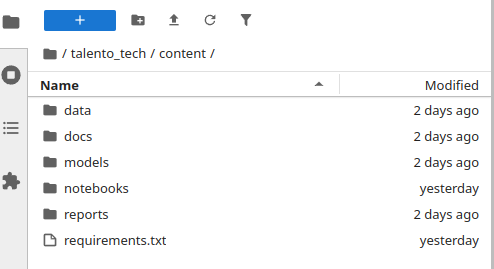
\includegraphics[width=0.7\linewidth]{cookiecutter}
	\caption[Estructura cookiecutter]{Estructura cookiecutter para proyecto de ciencia de datos}
	\label{fig:cookiecutter}
\end{figure}


\subsection{Enriquecimiento de la informaci\'on}

Se ha mejorado el conjunto de datos adicionando los a\~nos 2023, 2024 y los meses de enero y febrero para el 2025. Se ha utilizado t\'ecnicas de web scrapping para obtener la informaci\'on adicional.


\begin{minted}[]{python}
# Import necessary libraries
import os
import csv
import requests
from pprint import pprint

# Set show information about API request
VERBOSE = True

# Define API endpoints for getting available years, products, and countries
api_list_template = 'https://api.iea.org/mes/list/%s'

# Define API endpoint for getting monthly data for a specific country, year, month, and product
api_information_template = 'https://api.iea.org/mes/latest/month?COUNTRY=%s&YEAR=%s&MONTH=%s&PRODUCT=%s&share=true'

# Get lists of available years, products, and countries from the API
years = requests.get(api_list_template % 'YEAR').json()
products = requests.get(api_list_template % 'PRODUCT').json()
countries = requests.get(api_list_template % 'COUNTRY').json()

# Define the header row for the CSV file that will store the data
header = [
'COUNTRY',           # Name of the country
'CODE_TIME',         # A code that represents the month and year (e.g., JAN2010 for January 2010)
'TIME',              # The month and year in a more human-readable format (e.g., January 2010)
'YEAR',              # The year of the data point
'MONTH',             # The month of the data point as a number (1-12)
'MONTH_NAME',        # The month of the data point as a string (e.g., January)
'PRODUCT',           # The type of energy product (e.g., Hydro, Wind, Solar)
'VALUE',             # The amount of electricity generated in gigawatt-hours (GWh)
'DISPLAY_ORDER',     # The order in which the products should be displayed
'yearToDate',        # The amount of electricity generated for the current year up to the current month in GWh
'previousYearToDate',# The amount of electricity generated for the previous year up to the current month in GWh
'share'              # The share of the product in the total electricity generation for the country in decimal format
]

# Check if data.csv file exists
if os.path.isfile('data.csv'):
	# Check if file is empty 
	if os.stat('data.csv').st_size != 0:
		# Read CSV file and get the last line of it
		with open('data.csv', 'r') as csv_file:
		last_line = csv_file.readlines()[-1].split(',')

		# Extract the information from the last line get their index values
		index_last_year = years.index(int(last_line[3]))
		index_last_month = int(last_line[4])
		index_last_country = countries.index(last_line[0])
		index_last_product = products.index(last_line[6]) + 1

	else:
		# If CSV file is empty 
		index_last_year, index_last_month, index_last_country, index_last_product = 0, 1, 0, 0

# Open CSV file for writing
with open('data.csv', 'a+', newline='') as csv_file:
	writer = csv.DictWriter(csv_file, fieldnames=header)

	# Scrape the data and write it to the CSV file
	for year in years[index_last_year:]:
		for month in range(index_last_month, 13):
			for country in countries[index_last_country:]:
				# Replace apostrophes in the country name with %27 to create a valid URL
				country = country.replace('\'', '%27')

				for product in products[index_last_product:]:
					# Send an API request to get monthly data for the current country, year, month and product
					response = requests.get(
						api_information_template % (country, year, month, product)
					)

					# Check if the API response is OK
					if response.ok:
						# Parse the response JSON
						response = response.json()


						# if response has data
						if len(response['latest']) != 0:

							print(response)

							# Create a dictionary of the data to write to the CSV file
							result = dict()

							# Extract the data from the response and add it to the result dictionary
							for key in response['latest'][0].keys():
								result[key] = response['latest'][0][key]

							# Add year-to-date, previous-year-to-date and share data to the result dictionary
							result['yearToDate'] = response['yearToDate']
							result['previousYearToDate'] = response['previousYearToDate']
							result['share'] = response['share']

							# Write the result dictionary to the CSV file
							writer.writerow(result)

							# If verbose mode is on, print the result for this month
							if VERBOSE:
								pprint(result, sort_dicts=False)
								print('_________________________')

		index_last_product = 0
		index_last_month = 1
		index_last_country = 0
\end{minted}

En la figura \ref{fig:scapping1} se muestra el web scrapping en funcionamiento descargando la informaci\'on de los a\~nos faltantes.

\begin{figure}
	\centering
	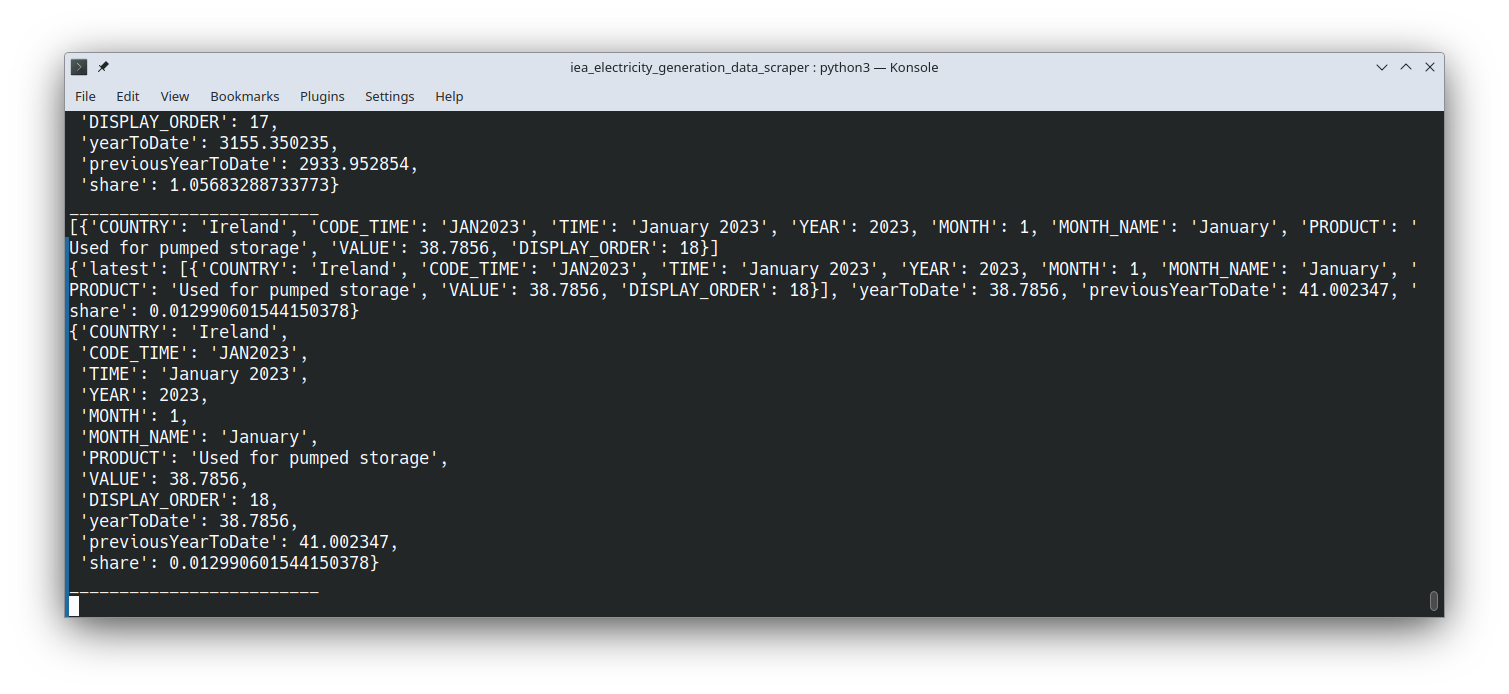
\includegraphics[width=0.9\linewidth]{scapping_1}
	\caption[Web scrapping]{Web scrapping descargando la informaci\'on de los a\~nos 2024 y 2025}
	\label{fig:scapping1}
\end{figure}


\subsection{Limpieza de datos}

Para la limpieza de datos se ha utilizado el archivo con la informaci\'on de producci\'on de energ\'ia electr\'ica desde el a\~no 2010 hasta 2025 inclusive. 

\subsubsection{Importaci\'on de las librer\'ias y asignaci\'on del directorio de trabajo}

\begin{minted}[]{python}
# import library
import pandas as pd
import os

# set default directory
os.chdir('/home/lbertel/code/talento_tech/content')
!ls
\end{minted}

\begin{verbatim}
data  docs  models  notebooks  reports	requirements.txt
\end{verbatim}

\subsubsection{Carga del archivo con datos en crudo}

\begin{minted}[]{python}
# load raw file
df_data_all_country = pd.read_csv('data/raw/data.csv')

# print all data
df_data_all_country.info()
\end{minted}

\begin{verbatim}
<class 'pandas.core.frame.DataFrame'>
RangeIndex: 213138 entries, 0 to 213137
Data columns (total 12 columns):
#   Column              Non-Null Count   Dtype  
---  ------              --------------   -----  
0   COUNTRY             213138 non-null  object 
1   CODE_TIME           213138 non-null  object 
2   TIME                213138 non-null  object 
3   YEAR                213138 non-null  int64  
4   MONTH               213138 non-null  int64  
5   MONTH_NAME          213138 non-null  object 
6   PRODUCT             213138 non-null  object 
7   VALUE               213138 non-null  float64
8   DISPLAY_ORDER       213138 non-null  int64  
9   yearToDate          213138 non-null  float64
10  previousYearToDate  196016 non-null  float64
11  share               213138 non-null  float64
dtypes: float64(4), int64(3), object(5)
memory usage: 19.5+ MB
\end{verbatim}

\subsubsection{Recuperar los registros asociados al pa\'is Colombia}

\begin{minted}[]{python}
# select row with COUNTRY is equal Colombia
df_data_colombia = df_data_all_country[df_data_all_country['COUNTRY'] == 'Colombia']

# print first record of Colombia
df_data_colombia.head(10)

# size dataframe
len(df_data_colombia)
\end{minted}

\begin{verbatim}
3104
\end{verbatim}


\subsubsection{Recuperar los registros asociados al pa\'is Colombia}

\begin{minted}[]{python}
	# select row with COUNTRY is equal Colombia
	df_data_colombia = df_data_all_country[df_data_all_country['COUNTRY'] == 'Colombia']
	
	# print first record of Colombia
	df_data_colombia.head(10)
	
	# size dataframe
	len(df_data_colombia)
\end{minted}

\begin{verbatim}
	3104
\end{verbatim}

\subsubsection{Eliminar categorias no necesarias en el estudio}

\begin{minted}[]{python}
# show columns after delete
print(df_data_colombia.columns)

# delete columns
df_temp = df_data_colombia.drop(['COUNTRY', 'CODE_TIME', 'TIME', 'MONTH_NAME', 'DISPLAY_ORDER', 'yearToDate', 'previousYearToDate', 'share'], axis=1)

# show columns before delete
print(df_temp.columns)
print('')
print('---------------------------------')
print('')

df_temp.info()
\end{minted}

\begin{verbatim}
Index(['COUNTRY', 'CODE_TIME', 'TIME', 'YEAR', 'MONTH', 'MONTH_NAME',
'PRODUCT', 'VALUE', 'DISPLAY_ORDER', 'yearToDate', 'previousYearToDate',
'share'],
dtype='object')
Index(['YEAR', 'MONTH', 'PRODUCT', 'VALUE'], dtype='object')

---------------------------------

<class 'pandas.core.frame.DataFrame'>
Index: 3104 entries, 46557 to 212133
Data columns (total 4 columns):
#   Column   Non-Null Count  Dtype  
---  ------   --------------  -----  
0   YEAR     3104 non-null   int64  
1   MONTH    3104 non-null   int64  
2   PRODUCT  3104 non-null   object 
3   VALUE    3104 non-null   float64
dtypes: float64(1), int64(2), object(1)
memory usage: 121.2+ KB
\end{verbatim}

\subsubsection{Eliminar registros con valores nulos y que en la categor\'ia PRODUCT tenga totales}

\begin{minted}[]{python}
# delete row with null values
len(df_temp)
df_without_null = df_temp.dropna(how='any')

# size dataframe without null
len(df_without_null)

# eliminate row with PRODUCT containt Total
filter_total = df_without_null[~df_without_null['PRODUCT'].str.contains('Total', case=False, na=False)]

len(filter_total)
\end{minted}

\begin{verbatim}
2706
\end{verbatim}

\subsubsection{Guardar el dataframe en un archivo}

\begin{minted}[]{python}
# save the new dataframe
filter_total.to_csv('data/processed/colombia_data.csv', index=False)

# information dataframe
filter_total.info()
\end{minted}

\begin{verbatim}
<class 'pandas.core.frame.DataFrame'>
Index: 2706 entries, 46557 to 212133
Data columns (total 4 columns):
#   Column   Non-Null Count  Dtype  
---  ------   --------------  -----  
0   YEAR     2706 non-null   int64  
1   MONTH    2706 non-null   int64  
2   PRODUCT  2706 non-null   object 
3   VALUE    2706 non-null   float64
dtypes: float64(1), int64(2), object(1)
memory usage: 105.7+ KB
\end{verbatim}

\subsubsection{Mostrar informaci\'on del dataset ya limpio}

\begin{minted}[]{python}
# dimension of dataframe
filter_total.shape

# missing values
filter_total.isnull().sum(axis=0)
\end{minted}

\begin{verbatim}
YEAR       0
MONTH      0
PRODUCT    0
VALUE      0
dtype: int64
\end{verbatim}

\subsection{An\'alisis multidimensional}

\subsubsection{Importacio\'on de librer\'ias y Carga del archivo de trabajo}

\begin{minted}[]{python}
# import library
import os
import pandas as pd
import numpy as np
import seaborn as sns
import matplotlib
import matplotlib.pyplot as plt

# set default directory
os.chdir('/home/lbertel/code/talento_tech/content')

# set style matplotlib
plt.style.use('tableau-colorblind10')

# load data
colombia_df = pd.read_csv('data/processed/colombia_data.csv')
colombia_df.head(10)
\end{minted}

{\tt
\begin{tabular}{lllll}
	 & YEAR & MONTH & PRODUCT                    & VALUE    \\
	0   & 2014 & 1     & Hydro                      & 3903.977 \\
	1   & 2014 & 1     & Wind                       & 5.648    \\
	2   & 2014 & 1     & Solar                      & 1.065    \\
	3   & 2014 & 1     & Coal                       & 521.938  \\
	4   & 2014 & 1     & Oil                        & 139.219  \\
	5   & 2014 & 1     & Natural gas                & 1031.146 \\
	6   & 2014 & 1     & Combustible renewables     & 99.721   \\
	7   & 2014 & 1     & Net electricity production & 5702.714 \\
	8   & 2014 & 1     & Electricity supplied       & 5555.847 \\
	9   & 2014 & 1     & Distribution losses        & 536.164 
\end{tabular}
}

\subsubsection{Cantidad de energía clasificada según tipo}

\begin{minted}[]{python}
# energy clasification dataset
order = colombia_df.groupby('PRODUCT').mean()['VALUE'].sort_values(ascending=False).index

fig, ax = plt.subplots(figsize=(8, 8))
fig.suptitle('Cantidad de energía clasificada según tipo')

sns.barplot(data=colombia_df, x='VALUE', y='PRODUCT', ax=ax, estimator='mean', errorbar=None, order=order)
ax.set_xlabel('Cantidad de Energía [GWh]')
ax.set_ylabel('Tipo de energía')

plt.tight_layout()
\end{minted}

\begin{figure}[t]
	\centering
	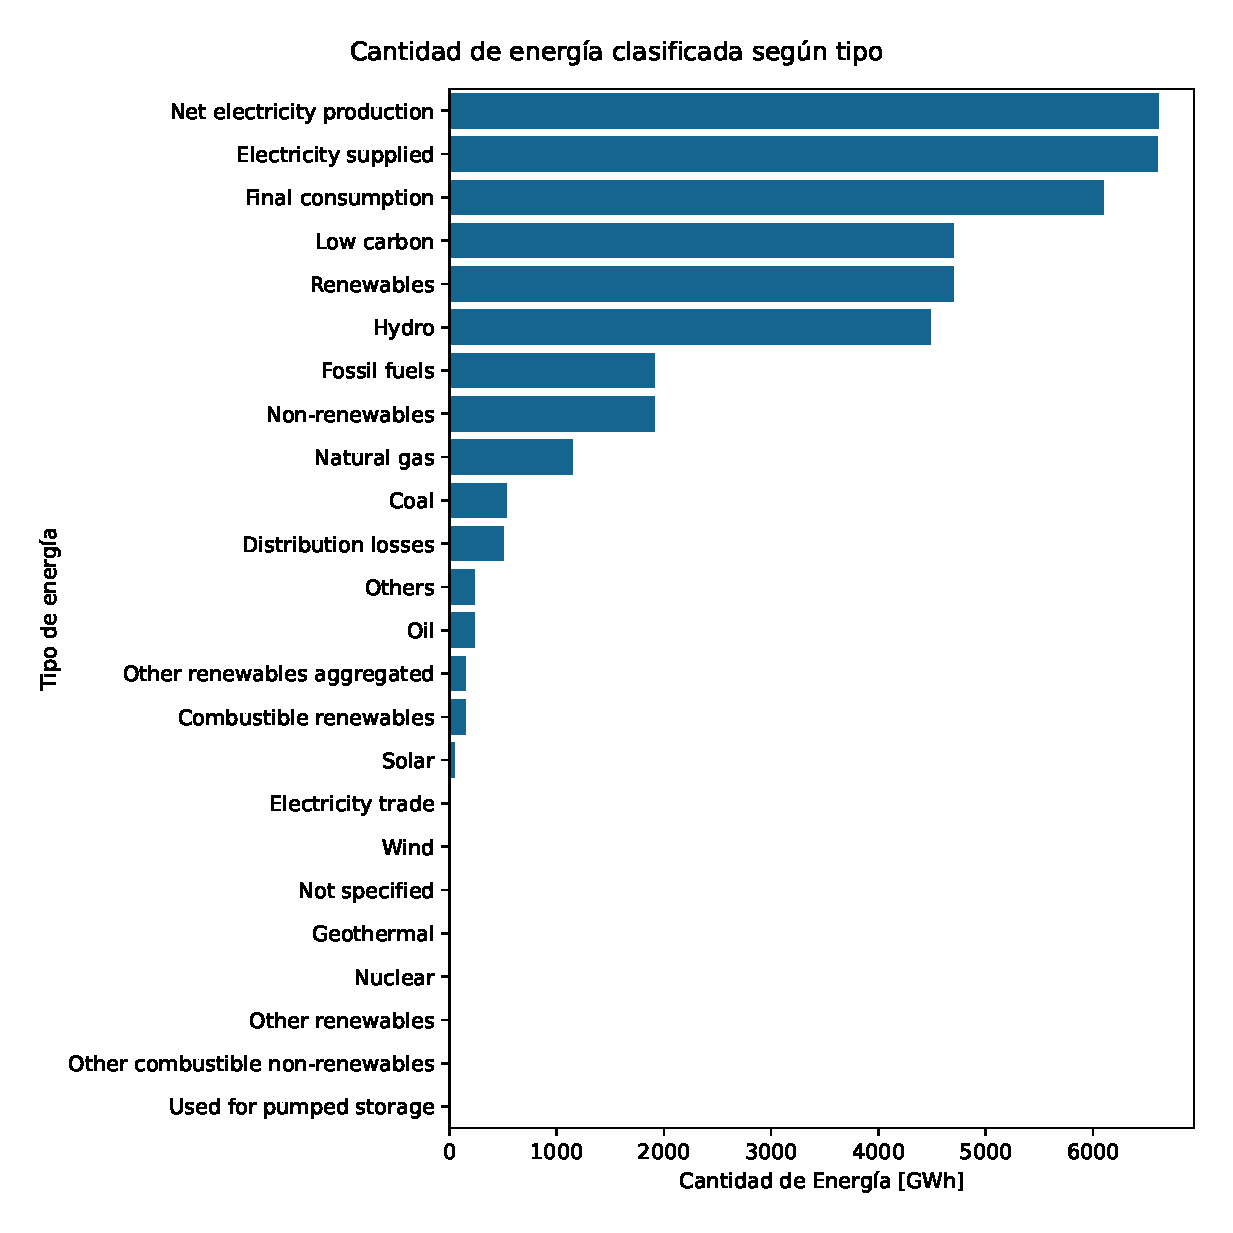
\includegraphics[width=0.7\linewidth]{fig_3}
	\caption{Cantidad de energ\'ia clasificada por tipo}
	\label{fig:fig3}
\end{figure}

\subsubsection{Evolución de la producción neta de energía en Colombia (Resolución Anual)}

\begin{minted}[]{python}
# energy production 2014-2025
filt = (colombia_df['PRODUCT'] == 'Net electricity production')
df_net = colombia_df.loc[filt]
fig, ax = plt.subplots(figsize=(10, 4))
fig.suptitle('Evolución de la producción neta de energía en Colombia (Resolución Anual)')

sns.pointplot(data=df_net, x='YEAR', y='VALUE', ax=ax, estimator='mean', errorbar=None)
ax.set_xlabel('Año')
ax.set_ylabel('Energía Promedio [GWh]')

plt.tight_layout()
\end{minted}

\begin{figure}[t]
	\centering
	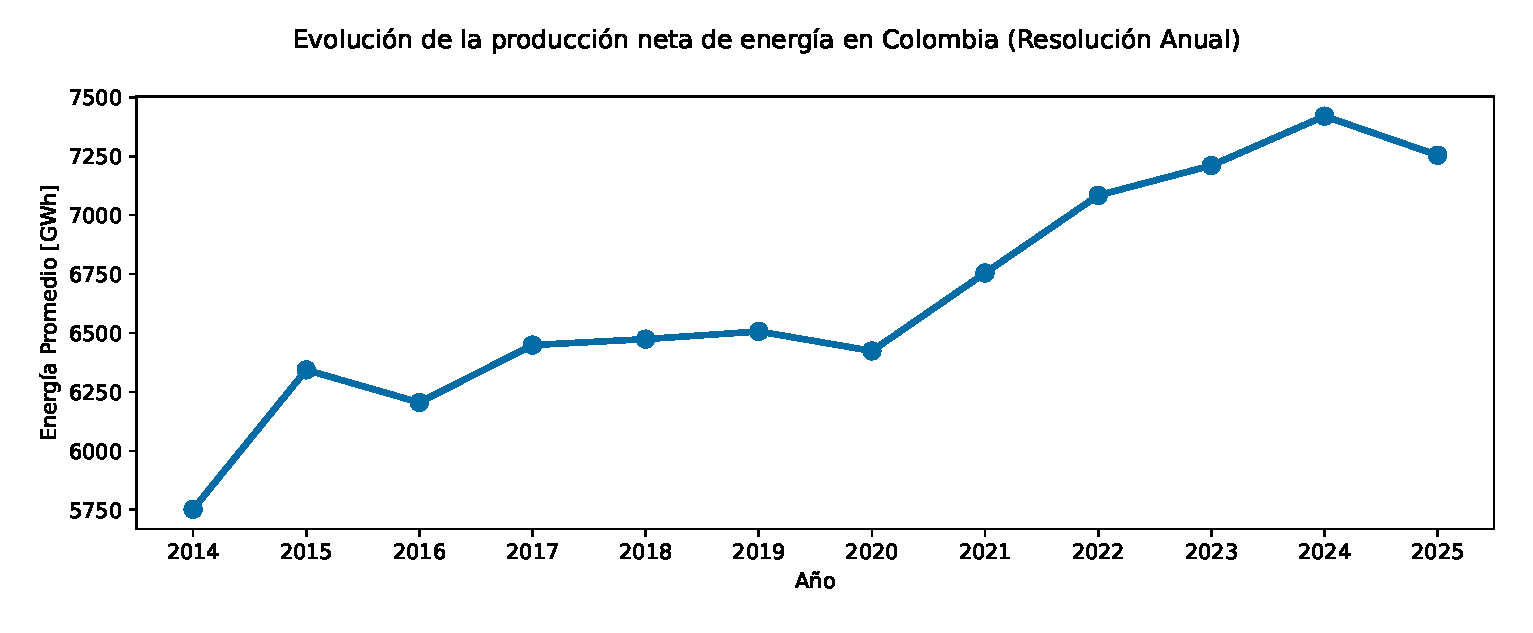
\includegraphics[width=0.7\linewidth]{fig_4}
	\caption{Evolución de la producción neta de energía en Colombia}
	\label{fig:fig4}
\end{figure}

\subsubsection{Producción neta mensual de energía en Colombia}

\begin{minted}[]{python}
fig, ax = plt.subplots(figsize=(10, 4))
fig.suptitle('Producción neta mensual de energía en Colombia')

sns.pointplot(data=df_net, x='MONTH', y='VALUE', ax=ax, estimator='mean', errorbar=None)
ax.set_xlabel('Mes')
ax.set_ylabel('Energía Promedio [GWh]')
ax.set_ylim([5000, 8000])

plt.tight_layout()
\end{minted}

\begin{figure}[t]
	\centering
	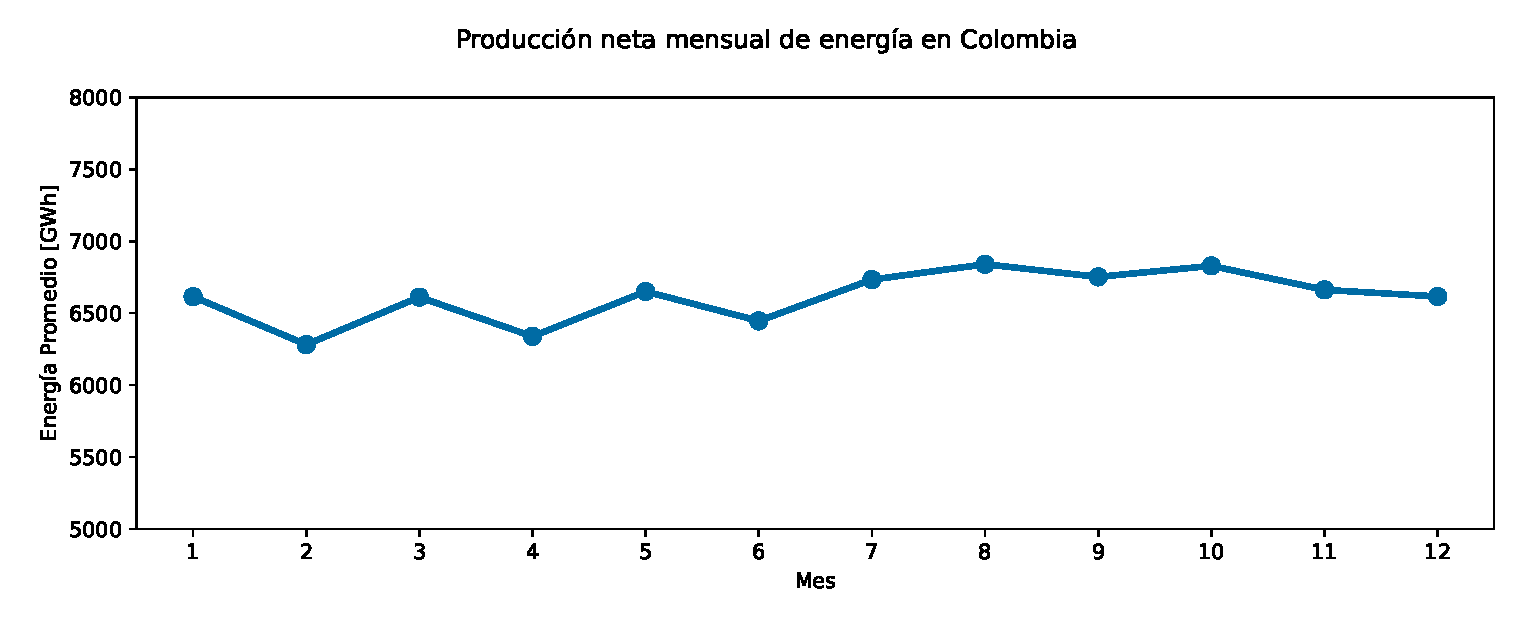
\includegraphics[width=0.7\linewidth]{fig_5}
	\caption{Producción neta mensual de energía en Colombia}
	\label{fig:fig5}
\end{figure}

\subsubsection{Matriz energética de Colombia}

\begin{minted}[]{python}
# select 
filt = ['Wind', 'Solar', 'Other renew. agg.', 'Others', 'Nuclear', 'Natural gas', 'Hydro', 'Coal']
df_gen = colombia_df[colombia_df['PRODUCT'].isin(filt)]

matrix = df_gen.groupby('PRODUCT').sum()['VALUE'].sort_values(ascending=False)
matrix
\end{minted}

\begin{verbatim}
PRODUCT
Hydro          601415.683695
Natural gas    153592.481385
Coal            71158.873666
Others          31527.442435
Solar            7138.600132
Wind              629.372654
Nuclear             0.000000
Name: VALUE, dtype: float64
\end{verbatim}

\begin{minted}[]{python}
labels = matrix.index

fig, ax = plt.subplots(figsize=(10, 4))
fig.suptitle('Matriz energética de Colombia')

ax.pie(x=matrix, labels=labels, autopct='%.0f%%', rotatelabels=True,startangle=180, colors=sns.color_palette("pastel"));
plt.legend(loc='center left', bbox_to_anchor=(1, 0.5), labels=["{} - {:.2f}%".format(i,j/sum(matrix)*100) for i,j in zip(labels,matrix)], frameon=False)

plt.tight_layout()
\end{minted}

\begin{figure}[t]
	\centering
	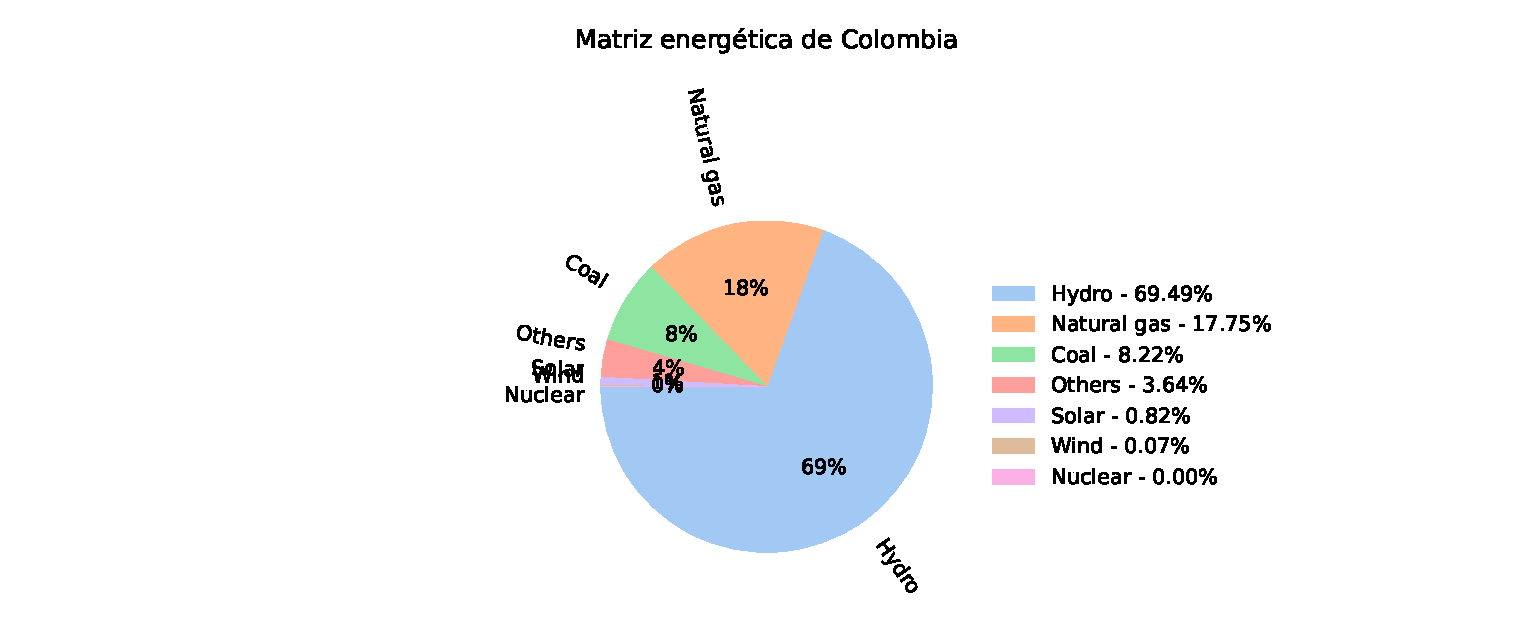
\includegraphics[width=1\linewidth]{fig_6}
	\caption{Matriz energética de Colombia}
	\label{fig:fig6}
\end{figure}

\subsubsection{Energía según tipo de generación}

\begin{minted}[]{python}
order = df_gen.groupby('PRODUCT').mean()['VALUE'].sort_values(ascending=False).index

fig, ax = plt.subplots(figsize=(10, 4))
fig.suptitle('Energía según tipo de generación')

sns.barplot(data=df_gen, x='VALUE', y='PRODUCT', ax=ax, estimator='mean', errorbar=None, order=order)
ax.set_xlabel('Energía promedio [GWh]')
ax.set_ylabel('Tipo de generación')

plt.tight_layout()
\end{minted}

\begin{figure}[t]
	\centering
	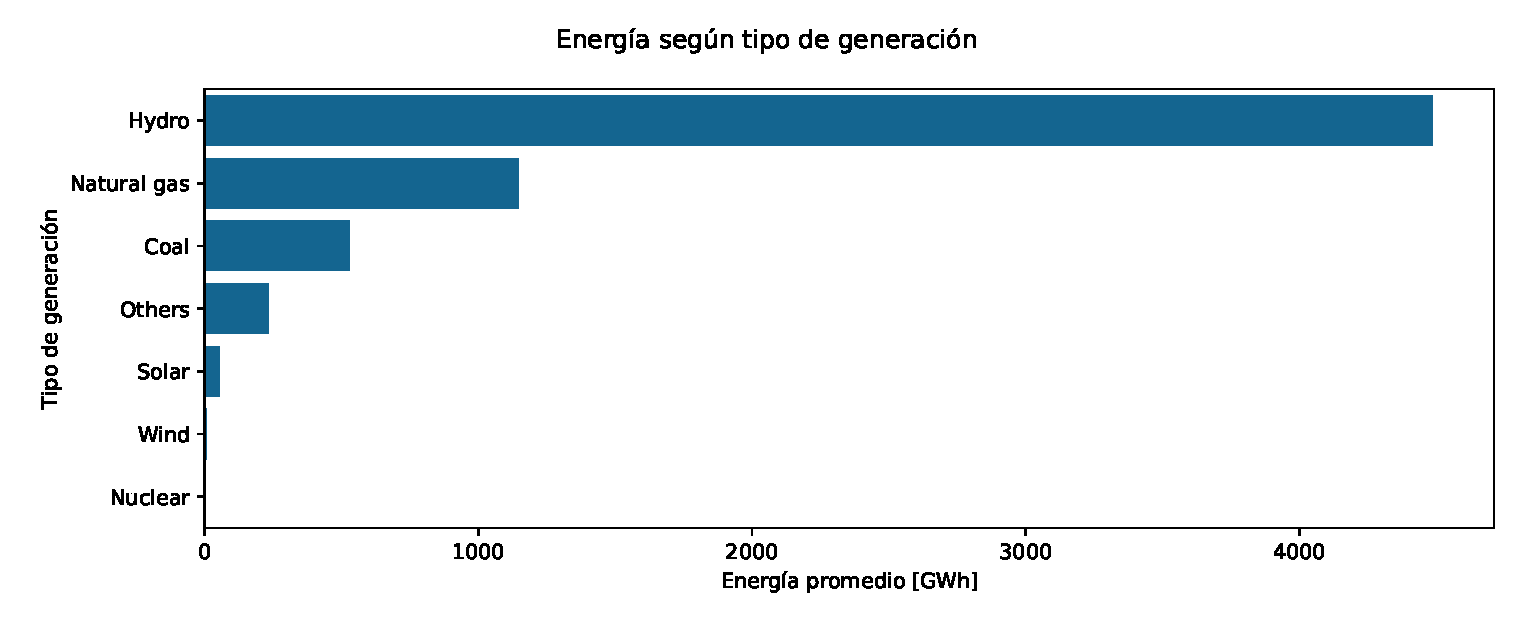
\includegraphics[width=0.7\linewidth]{fig_7}
	\caption{Energía según tipo de generación}
	\label{fig:fig7}
\end{figure}

\subsubsection{Evolución de la producción de energía en Colombia según tipo de generación}

\begin{minted}[]{python}
fig, ax = plt.subplots(figsize=(10, 4))
fig.suptitle('Evolución de la producción de energía en Colombia según tipo de generación')

sns.lineplot(data=df_gen, x='YEAR', y='VALUE', ax=ax, hue='PRODUCT', estimator='mean', errorbar=None, hue_order=order,)
ax.set_xlabel('Año')
ax.set_ylabel('Energía Promedio [GWh]')
ax.set_xlim([2014, 2025])
ax.set_ylim([0, 6000])
ax.legend(bbox_to_anchor=(1.02, 1), loc='upper left')

plt.tight_layout()
\end{minted}

\begin{figure}[t]
	\centering
	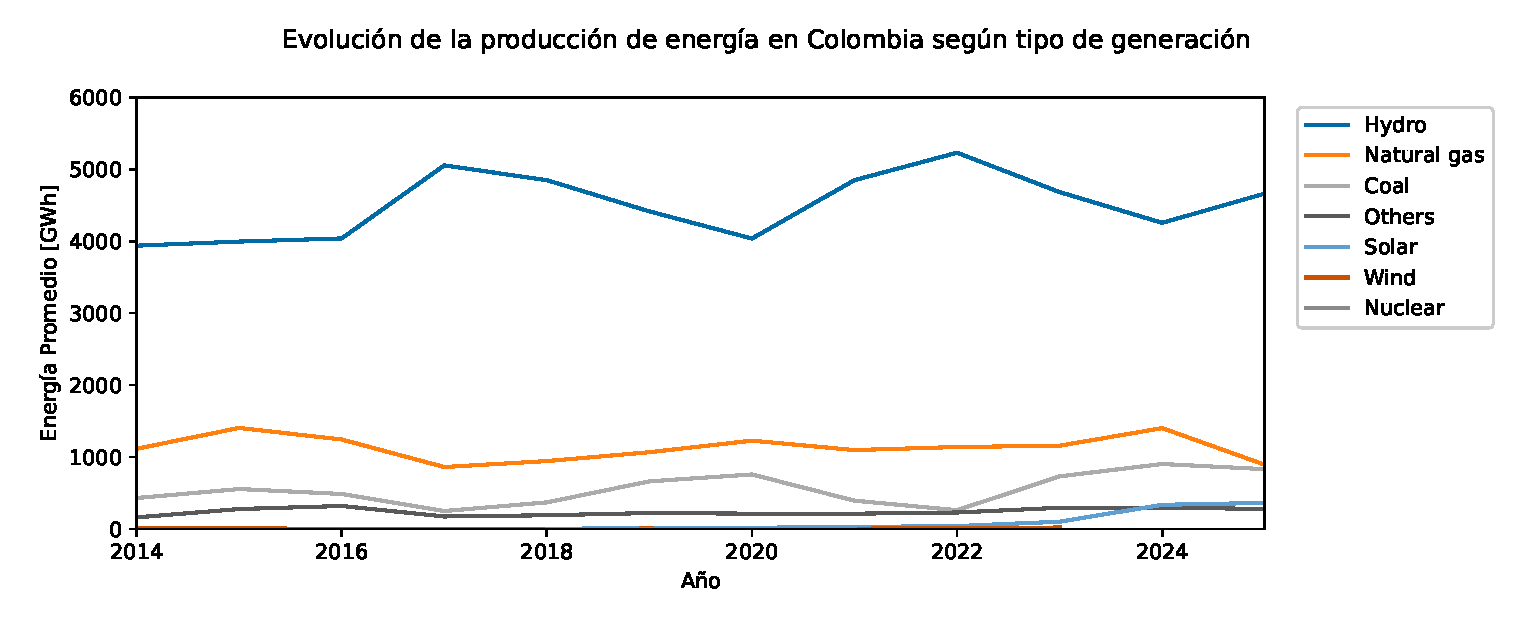
\includegraphics[width=0.7\linewidth]{fig_8}
	\caption{Evolución de la producción de energía en Colombia según tipo de generación}
	\label{fig:fig8}
\end{figure}

\subsubsection{Clasificaci\'on de la generaci\'on por tipo y a\~no}

\begin{minted}[]{python}
df_gen_year = df_gen.groupby(['YEAR','PRODUCT']).mean()
df_gen_year.sort_values(['YEAR', 'VALUE'], ascending=[True, False], inplace=True)
df_gen_year.head(14)
\end{minted}

{\tt
	\begin{tabular}{llll}
		&             & MONTH & VALUE       \\
		YEAR                  & PRODUCT     &       &             \\
		\multirow{6}{*}{2014} & Hydro       & 6.5   & 3937.424333 \\
		& Natural gas & 6.5   & 1113.783417 \\
		& Coal        & 6.5   & 429.340833  \\
		& Others      & 6.5   & 159.849250  \\
		& Wind        & 6.5   & 5.790167    \\
		& Solar       & 6.5   & 0.745583    \\
		\multirow{6}{*}{2015} & Hydro       & 6.5   & 3994.836750 \\
		& Natural gas & 6.5   & 1404.155417 \\
		& Coal        & 6.5   & 554.467500  \\
		& Others      & 6.5   & 276.451667  \\
		& Wind        & 6.5   & 5.624750    \\
		& Solar       & 6.5   & 0.745583    \\
		\multirow{2}{*}{2016} & Hydro       & 6.5   & 4038.266250 \\
		& Natural gas & 6.5   & 1243.133167
	\end{tabular}
}

\subsubsection{Evolución de la producción de energía en Colombia según tipo de generación}

\begin{minted}[]{python}
fig, ax = plt.subplots(figsize=(10, 4))
fig.suptitle('Evolución de la producción de energía en Colombia según tipo de generación')

sns.barplot(data=df_gen_year.reset_index(), x='YEAR', y='VALUE', hue='PRODUCT')
ax.set_xlabel('Año')
ax.set_ylabel('Energía Promedio [GWh]')
ax.legend(bbox_to_anchor=(1.02, 1), loc='upper left')

plt.tight_layout()
\end{minted}

\begin{figure}[t]
	\centering
	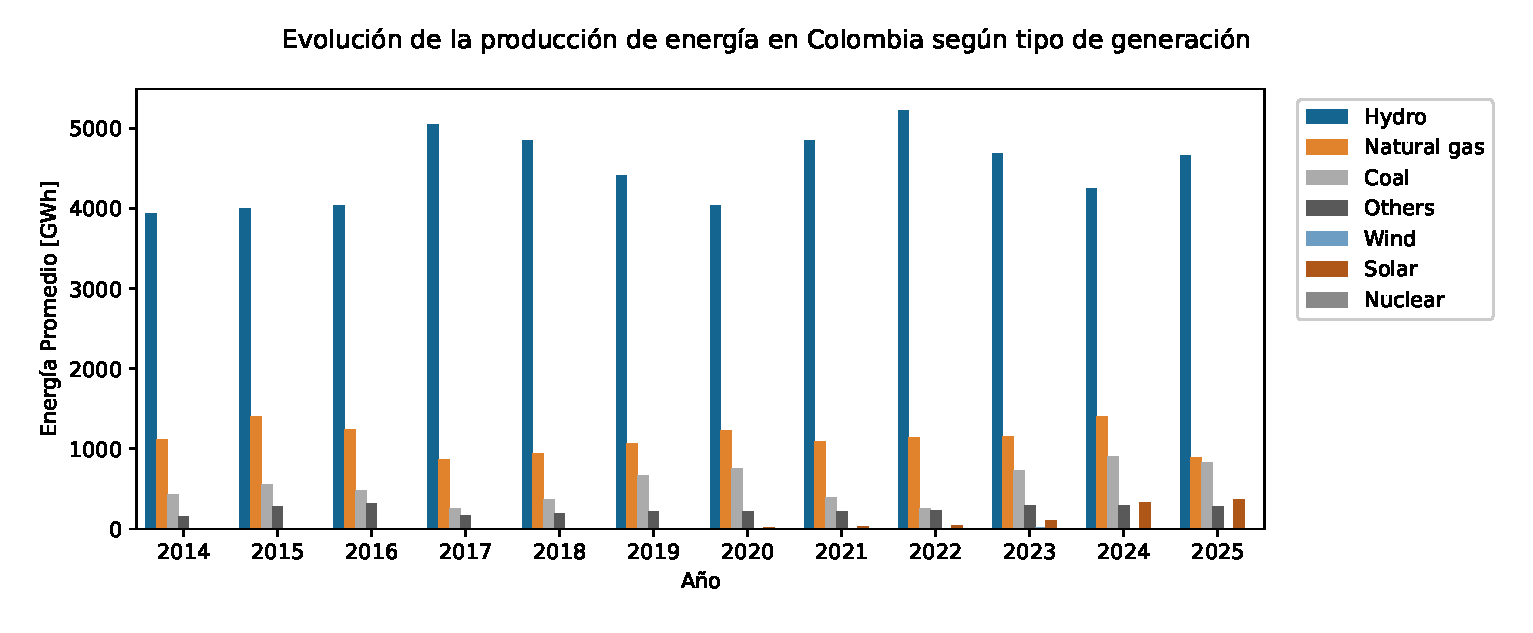
\includegraphics[width=0.7\linewidth]{fig_9}
	\caption{Evolución de la producción de energía en Colombia según tipo de generación}
	\label{fig:fig9}
\end{figure}

\subsubsection{Clasificaci\'on de las energ\'ias renovables y no renovables en Colombia}

\begin{minted}[]{python}
filt = ['Non-renewables', 'Renewables']
df_nr = colombia_df[colombia_df['PRODUCT'].isin(filt)]
df_nr.head()
\end{minted}

{\tt 
\begin{tabular}{lllll}
	&YEAR	&MONTH	&PRODUCT	&VALUE\\
12	&2014	&1	&Renewables	&4010.411\\
13	&2014	&1	&Non-renewables	&1692.303\\
30	&2014	&2	&Renewables	&3703.603\\
31	&2014	&2	&Non-renewables	&1661.258\\
48	&2014	&3	&Renewables	&4313.454\\
\end{tabular}
}

\subsubsection{Totales de energias renovables y no renovables}

\begin{minted}[]{python}
suma = df_nr.groupby('PRODUCT').sum()['VALUE'].sort_values(ascending=False)
suma
\end{minted}

{\tt
\begin{verbatim}
PRODUCT
Renewables        629704.771240
Non-renewables    256278.797486
Name: VALUE, dtype: float64
\end{verbatim}
}

\subsubsection{Proporción de producción de energía en Colombia Renovables vs No renovables}

\begin{minted}[]{python}
fig, ax = plt.subplots(figsize=(5, 5))
fig.suptitle('Proporción de producción de energía en Colombia Renovables vs No renovables')

ax.pie(x=suma, labels=suma.index, autopct='%.1f%%', startangle=90, colors=sns.color_palette("pastel"))

plt.tight_layout()	
\end{minted}

\begin{figure}[t]
	\centering
	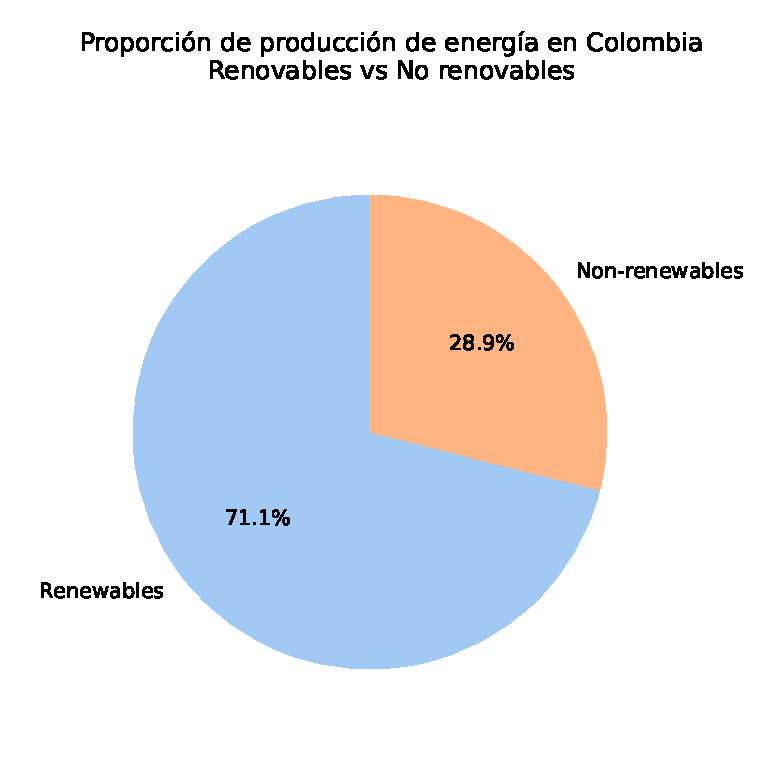
\includegraphics[width=0.7\linewidth]{fig_10}
	\caption{Proporción de producción de energía en Colombia Renovables vs No renovables}
	\label{fig:fig10}
\end{figure}

\subsubsection{Evolución de la producción de energía en Colombia. Renovable vs no renovable (2014-2025)}

\begin{minted}[]{python}
fig, ax = plt.subplots(figsize=(10, 4))
fig.suptitle('Evolución de la producción de energía en Colombia. Renovable vs no renovable (2014-2025)')

sns.lineplot(data=df_nr, x='YEAR', y='VALUE', ax=ax, hue='PRODUCT', estimator='mean', errorbar=None)
ax.set_xlabel('Año')
ax.set_ylabel('Energía Promedio [GWh]')
ax.set_xlim(2014, 2026)
ax.set_ylim([0, 6000])
ax.legend(bbox_to_anchor=(1.02, 1), loc='upper left')

plt.tight_layout()	
\end{minted}

\begin{figure}[t]
	\centering
	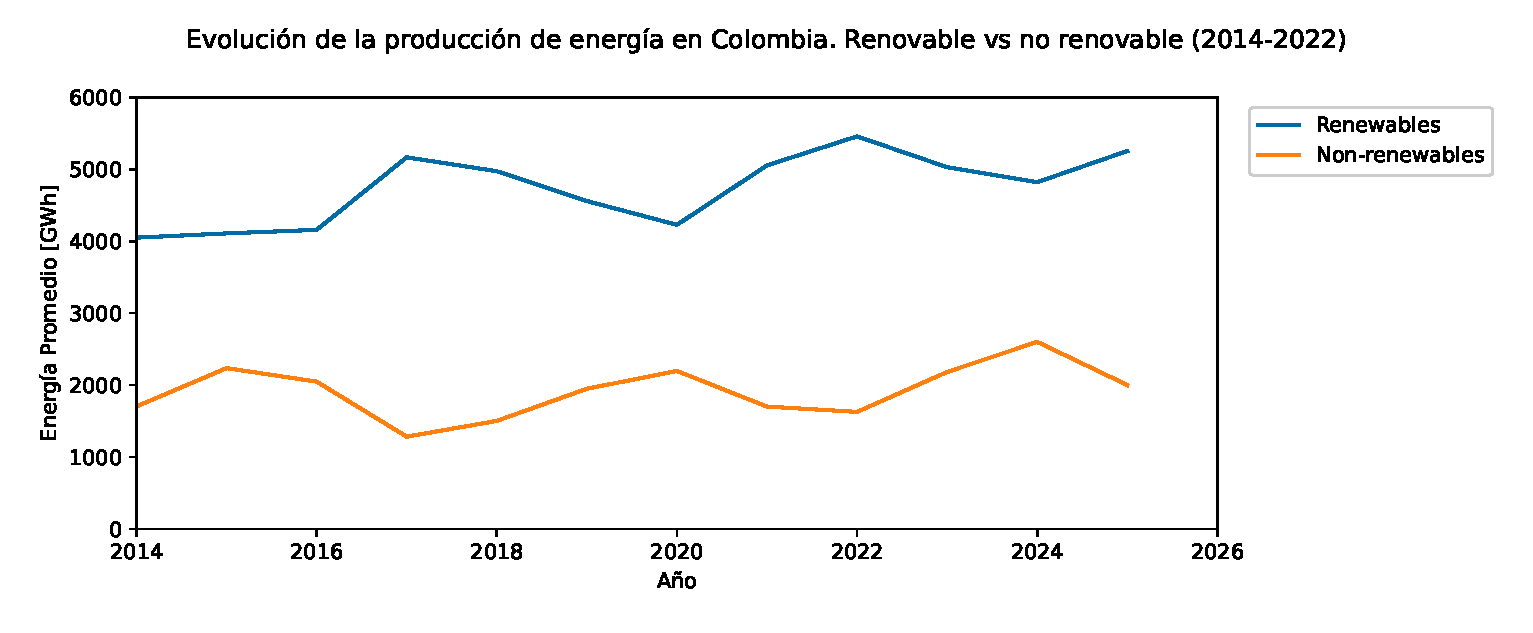
\includegraphics[width=0.7\linewidth]{fig_11}
	\caption{Evolución de la producción de energía en Colombia. Renovable vs no renovable (2014-2025)}
	\label{fig:fig11}
\end{figure}




\subsubsection{Descriminaci\'on de energ\'ias renovables}

\begin{minted}[]{python}
filt = ['Wind', 'Solar', 'Other renewables', 'Hydro', 'Geothermal', 'Combustible renewables']
df_ren = colombia_df[colombia_df['PRODUCT'].isin(filt)]
df_ren.head()
\end{minted}

{\tt
	\begin{tabular}{lllll}
		& YEAR & MONTH & PRODUCT                & VALUE    \\
		0  & 2014 & 1     & Hydro                  & 3903.977 \\
		1  & 2014 & 1     & Wind                   & 5.648    \\
		2  & 2014 & 1     & Solar                  & 1.065    \\
		6  & 2014 & 1     & Combustible renewables & 99.721   \\
		18 & 2014 & 2     & Hydro                  & 3598.260
	\end{tabular}
}

\subsubsection{Acumulado de energ\'ias renovables}

\begin{minted}[]{python}
	suma = df_ren.groupby('PRODUCT').sum()['VALUE'].sort_values(ascending=False)
	suma	
\end{minted}

\begin{verbatim}
	PRODUCT
	Hydro                     601415.683695
	Combustible renewables     20521.114759
	Solar                       7138.600132
	Wind                         629.372654
	Geothermal                     0.000000
	Other renewables               0.000000
	Name: VALUE, dtype: float64
\end{verbatim}

\subsubsection{Producción de energía de fuentes Renovables}

\begin{minted}[]{python}
order = df_ren.groupby('PRODUCT').mean()['VALUE'].sort_values(ascending=False).index

fig, ax = plt.subplots(figsize=(10, 4))
fig.suptitle('Producción de energía. Fuentes Renovables')

sns.barplot(data=df_ren, x='VALUE', y='PRODUCT', ax=ax, estimator='mean', errorbar=None, order=order)
ax.set_xlabel('Energía promedio [GWh]')
ax.set_ylabel('Tipo de generación')

plt.tight_layout()	
\end{minted}

\begin{figure}[t]
	\centering
	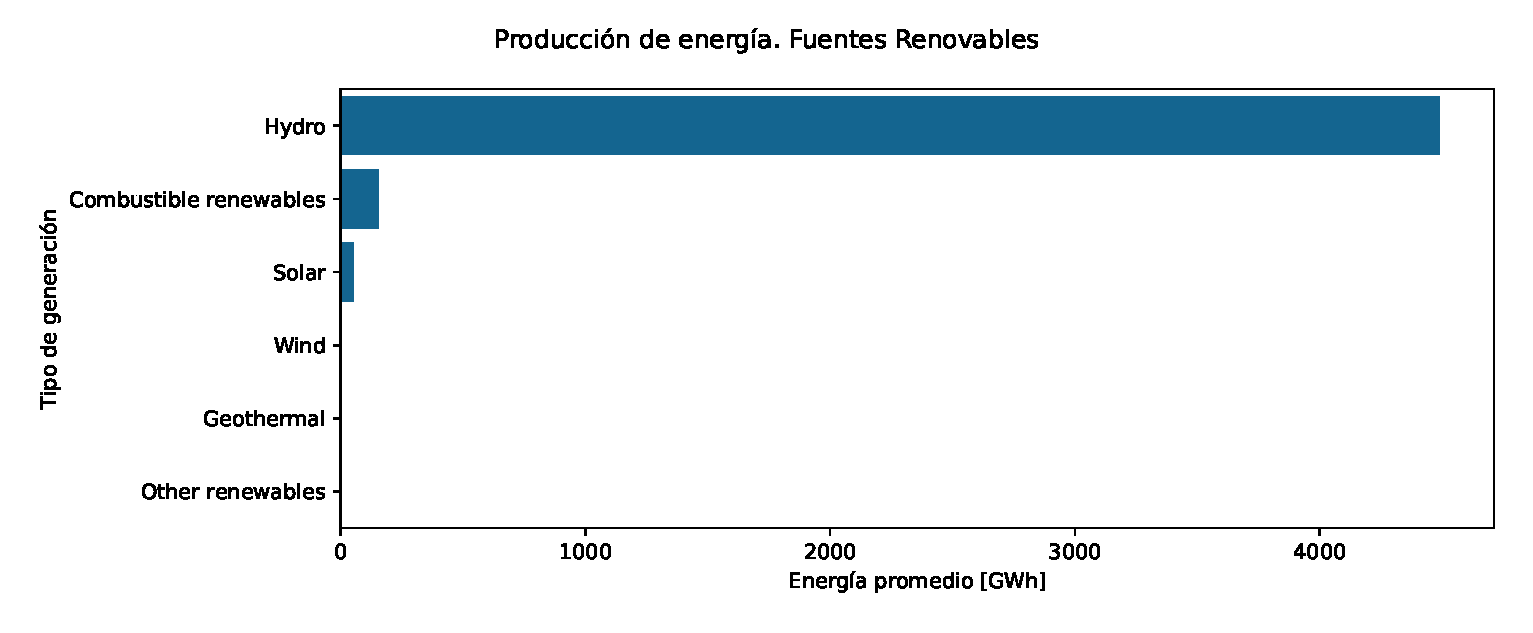
\includegraphics[width=0.7\linewidth]{fig_12}
	\caption{Producción de energía de fuentes Renovables}
	\label{fig:fig12}
\end{figure}


\subsubsection{Evolución de la producción de energía en Colombia. Fuentes Renovables (2014-2025)}

\begin{minted}[]{python}
fig, ax = plt.subplots(figsize=(10, 4))
fig.suptitle('Evolución de la producción de energía en Colombia. Fuentes Renovables (2014-2025)')

sns.lineplot(data=df_ren, x='YEAR', y='VALUE', ax=ax, hue='PRODUCT', estimator='mean', errorbar=None)
ax.set_xlabel('Año')
ax.set_ylabel('Energía Promedio [GWh]')
ax.set_xlim(2014, 2026)
ax.set_ylim([0, 6000])
ax.legend(bbox_to_anchor=(1.02, 1), loc='upper left')

plt.tight_layout()	
\end{minted}

\begin{figure}[t]
	\centering
	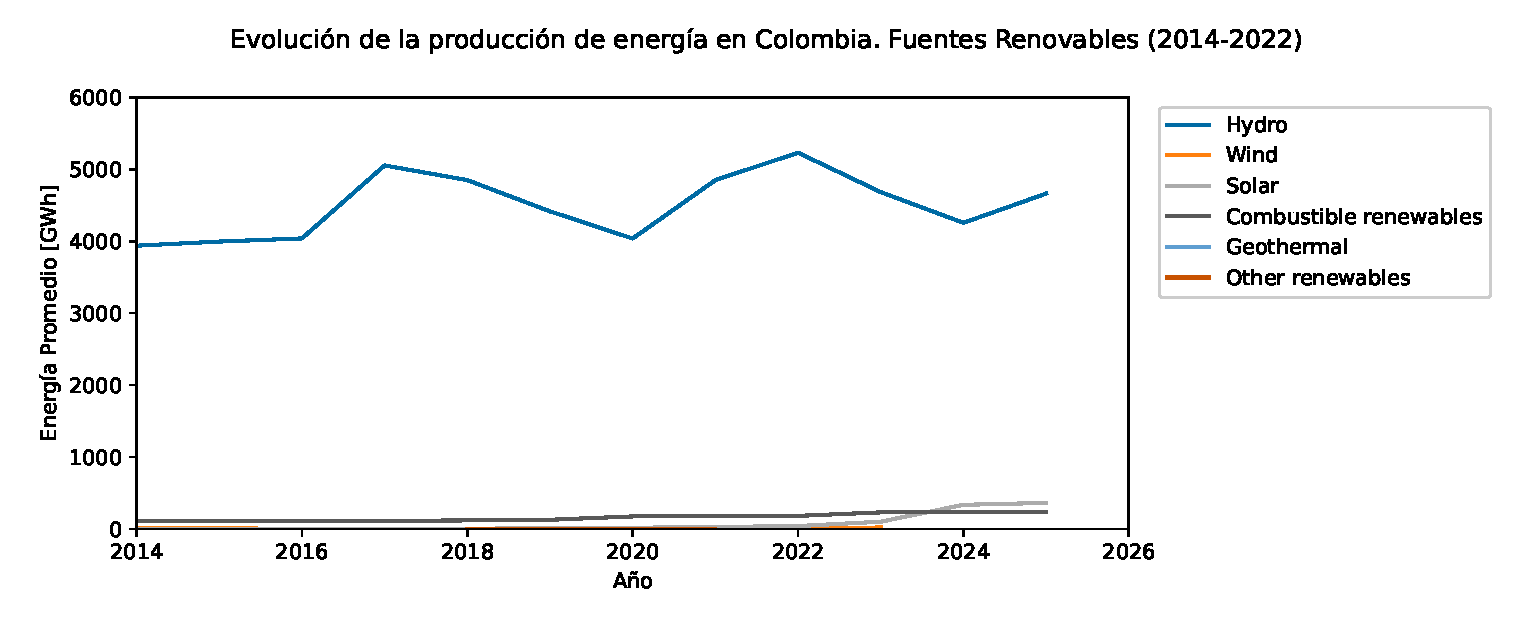
\includegraphics[width=0.7\linewidth]{fig_13}
	\caption{Evolución de la producción de energía en Colombia. Fuentes Renovables (2014-2025)}
	\label{fig:fig13}
\end{figure}

\subsubsection{Producción de energía. Fuentes Renovables. No hidraulica}

\begin{minted}[]{python}
order = df_ren[df_ren["PRODUCT"] != "Hydro"].groupby('PRODUCT').mean()['VALUE'].sort_values(ascending=False).index

fig, ax = plt.subplots(figsize=(10, 4))
fig.suptitle('Producción de energía. Fuentes Renovables. No hidraulica')

sns.barplot(data=df_ren[df_ren["PRODUCT"] != "Hydro"], x='VALUE', y='PRODUCT', ax=ax, estimator='mean', errorbar=None, order=order)
ax.set_xlabel('Energía promedio [GWh]')
ax.set_ylabel('Tipo de generación')

plt.tight_layout()	
\end{minted}

\begin{figure}[t]
	\centering
	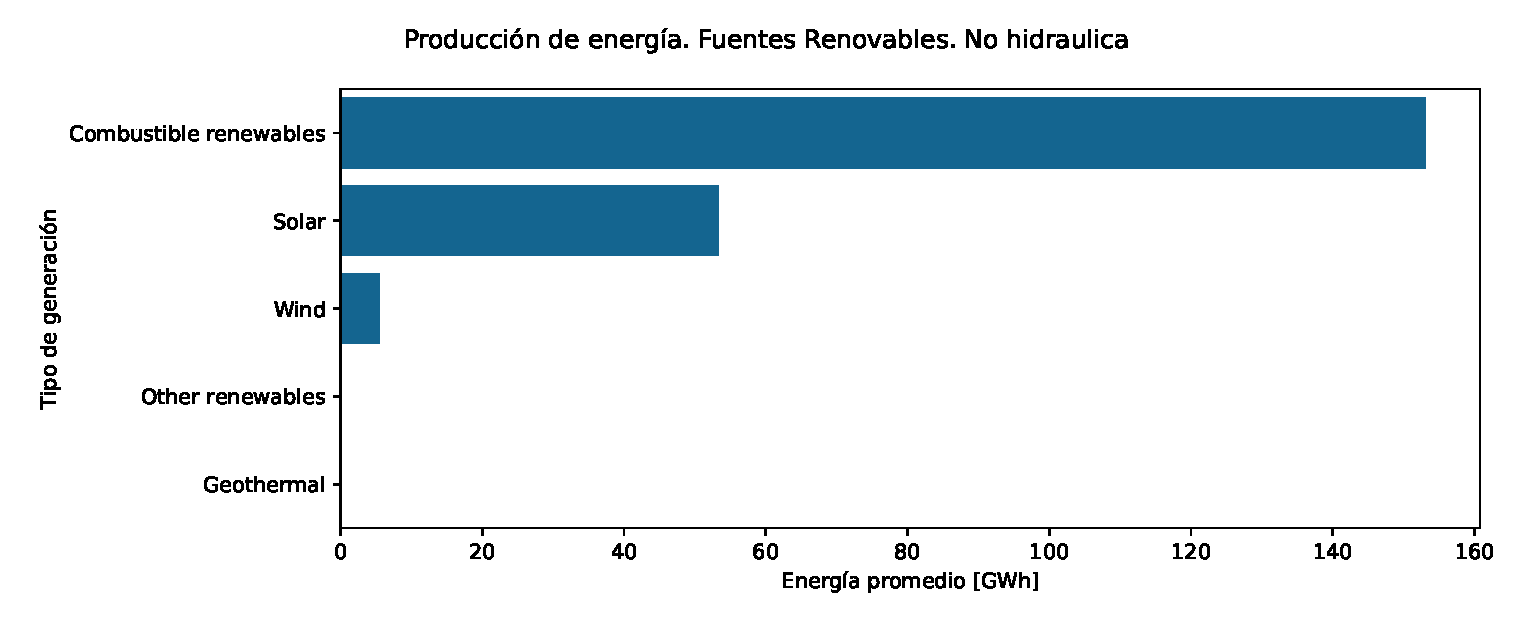
\includegraphics[width=0.7\linewidth]{fig_14}
	\caption{Producción de energía. Fuentes Renovables. No hidraulica}
	\label{fig:fig14}
\end{figure}


\subsubsection{Evolución de la producción de energía en Colombia fuentes renovables (2014-2025) no hidraulica}

\begin{minted}[]{python}
fig, ax = plt.subplots(figsize=(10, 4))
fig.suptitle('Evolución de la producción de energía en Colombia. Fuentes Renovables (2014-2022). No hidraulica')

sns.lineplot(data=df_ren[df_ren["PRODUCT"] != "Hydro"], x='YEAR', y='VALUE', ax=ax, hue='PRODUCT', estimator='mean', errorbar=None)
ax.set_xlabel('Año')
ax.set_ylabel('Energía Promedio [GWh]')
ax.set_xlim(2014, 2026)
# ax.set_ylim([0, 6000])
ax.legend(bbox_to_anchor=(1.02, 1), loc='upper left')

plt.tight_layout()
\end{minted}

\begin{figure}[t]
	\centering
	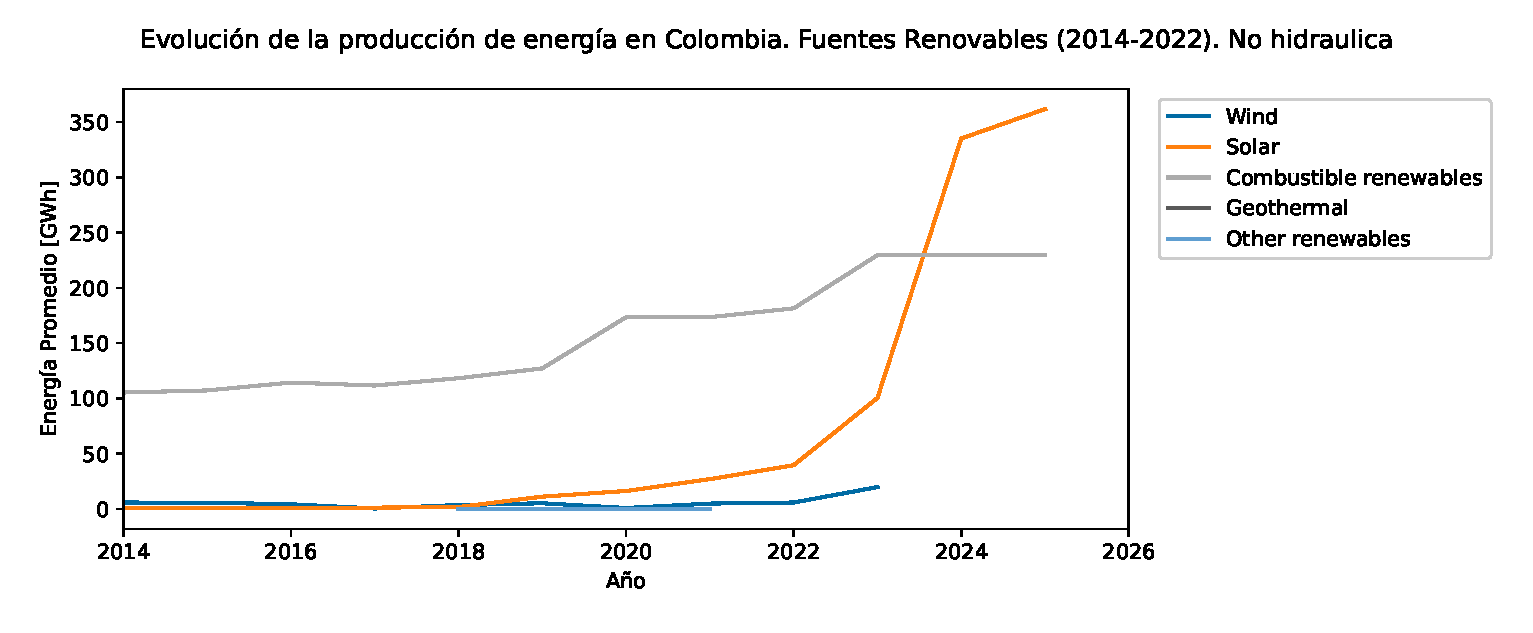
\includegraphics[width=0.7\linewidth]{fig_15}
	\caption{Producción de energía. Fuentes Renovables. No hidraulica}
	\label{fig:fig15}
\end{figure}


\subsubsection{Producción de energía de fuentes no renovables}

\begin{minted}[]{python}
filt = ['Coal', 'Natural gas', 'Fossil fuels', 'Nuclear']
df_notren = colombia_df[colombia_df['PRODUCT'].isin(filt)]
df_notren.head()	
\end{minted}

{\tt
\begin{tabular}{lllll}
	& YEAR & MONTH & PRODUCT      & VALUE    \\
	3  & 2014 & 1     & Coal         & 521.938  \\
	5  & 2014 & 1     & Natural gas  & 1031.146 \\
	17 & 2014 & 1     & Fossil fuels & 1692.303 \\
	21 & 2014 & 2     & Coal         & 413.943  \\
	23 & 2014 & 2     & Natural gas  & 1095.052
\end{tabular}
}

\subsubsection{Producción de energía de fuentes no renovables por tipo}

\begin{minted}[]{python}
suma = df_notren.groupby('PRODUCT').sum()['VALUE'].sort_values(ascending=False)
suma	
\end{minted}

\begin{verbatim}
PRODUCT
Fossil fuels    256278.797486
Natural gas     153592.481385
Coal             71158.873666
Nuclear              0.000000
Name: VALUE, dtype: float64
\end{verbatim}

\subsubsection{Producción de energía de fuentes no renovables}

\begin{minted}[]{python}
order = df_notren.groupby('PRODUCT').mean()['VALUE'].sort_values(ascending=False).index

fig, ax = plt.subplots(figsize=(10, 4))
fig.suptitle('Producción de energía. Fuentes No Renovables')

sns.barplot(data=df_notren, x='VALUE', y='PRODUCT', ax=ax, estimator='mean', errorbar=None, order=order)
ax.set_xlabel('Energía promedio [GWh]')
ax.set_ylabel('Tipo de generación')

plt.tight_layout()	
\end{minted}

\begin{figure}[t]
	\centering
	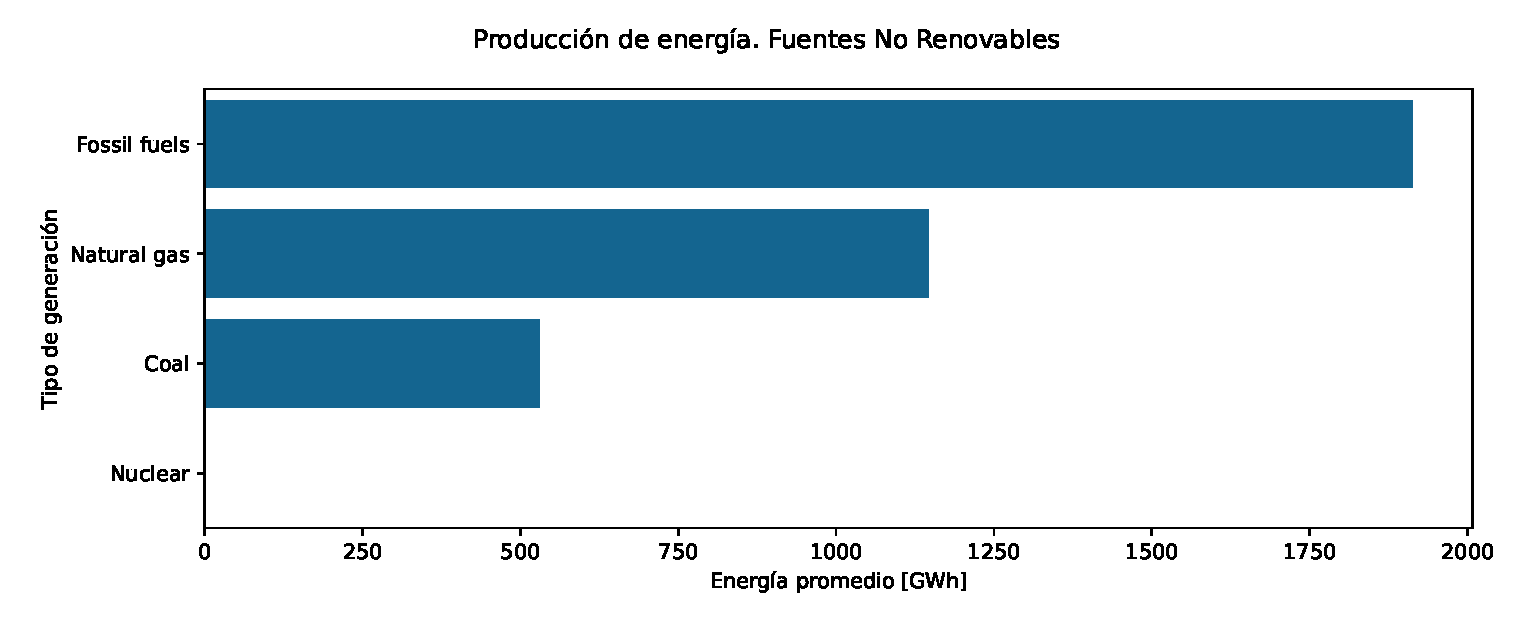
\includegraphics[width=0.7\linewidth]{fig_16}
	\caption{Producción de energía de fuentes no renovables}
	\label{fig:fig16}
\end{figure}

\subsubsection{Evolución de la producción de energía en Colombia de fuentes no renovables (2014-2025)}

\begin{minted}[]{python}
fig, ax = plt.subplots(figsize=(10, 4))
fig.suptitle('Evolución de la producción de energía en Colombia. Fuentes No Renovables (2014-2022)')

sns.lineplot(data=df_notren, x='YEAR', y='VALUE', ax=ax, hue='PRODUCT', estimator='mean', errorbar=None)
ax.set_xlabel('Año')
ax.set_ylabel('Energía Promedio [GWh]')
ax.set_xlim(2014, 2026)
# ax.set_ylim([0, 6000])
ax.legend(bbox_to_anchor=(1.02, 1), loc='upper left')

plt.tight_layout()
\end{minted}

\begin{figure}[t]
	\centering
	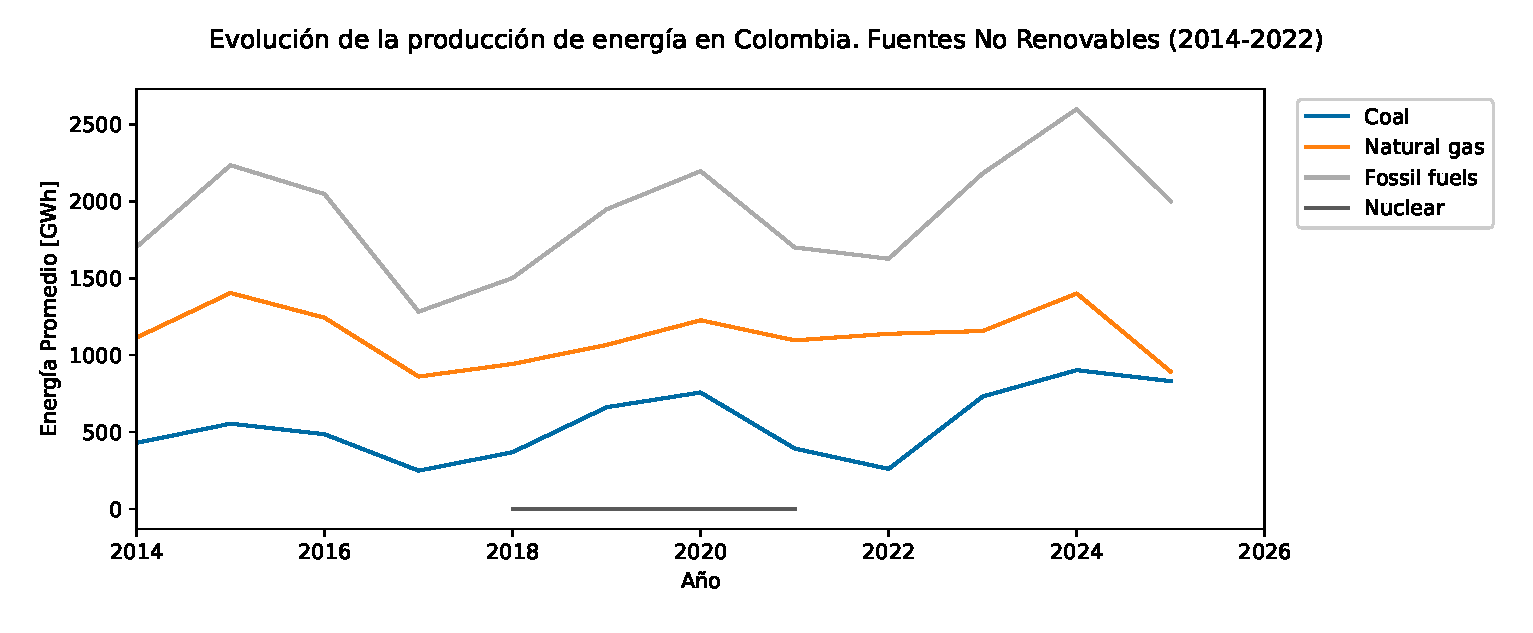
\includegraphics[width=0.7\linewidth]{fig_17}
	\caption{Evolución de la producción de energía en Colombia de fuentes no renovables (2014-2025)}
	\label{fig:fig17}
\end{figure}

\subsection{An\'alisis de datos con aprendizaje supervisado}

\subsubsection{Importaci\'on de librer\'ias y carga del archivo de trabajo}

\begin{minted}[]{python}
# import library
import pandas as pd
import numpy as np
from sklearn.linear_model import LinearRegression
import matplotlib.pyplot as plt
import seaborn as sns
import os
	
# set default directory
os.chdir('/home/lbertel/code/talento_tech/content')

# set style matplotlib
plt.style.use('tableau-colorblind10')

# load data
colombia_df = pd.read_csv('data/processed/colombia_data.csv')
colombia_df.head(10)
\end{minted}

{\tt
	\begin{tabular}{lllll}
		& YEAR & MONTH & PRODUCT                    & VALUE    \\
		0   & 2014 & 1     & Hydro                      & 3903.977 \\
		1   & 2014 & 1     & Wind                       & 5.648    \\
		2   & 2014 & 1     & Solar                      & 1.065    \\
		3   & 2014 & 1     & Coal                       & 521.938  \\
		4   & 2014 & 1     & Oil                        & 139.219  \\
		5   & 2014 & 1     & Natural gas                & 1031.146 \\
		6   & 2014 & 1     & Combustible renewables     & 99.721   \\
		7   & 2014 & 1     & Net electricity production & 5702.714 \\
		8   & 2014 & 1     & Electricity supplied       & 5555.847 \\
		9   & 2014 & 1     & Distribution losses        & 536.164 
	\end{tabular}
}

\subsubsection{Regresión lineal de la producción eléctrica en Colombia}

\begin{minted}[]{python}
# Group by year and add up total production
df_total = colombia_df.groupby('YEAR')['VALUE'].sum().reset_index()

# Create regression model
X = df_total[['YEAR']]
y = df_total['VALUE']
model = LinearRegression().fit(X, y)

# Predictions
df_total['PREDICCION'] = model.predict(X)

# Show results
plt.figure(figsize=(10,6))
sns.scatterplot(data=df_total, x='YEAR', y='VALUE', label='Real')
sns.lineplot(data=df_total, x='YEAR', y='PREDICCION', color='red', label='Predicción')
plt.title('Regresión lineal de la producción eléctrica en Colombia')
plt.grid(True)
plt.legend()
plt.show()
\end{minted}

\begin{figure}[t]
	\centering
	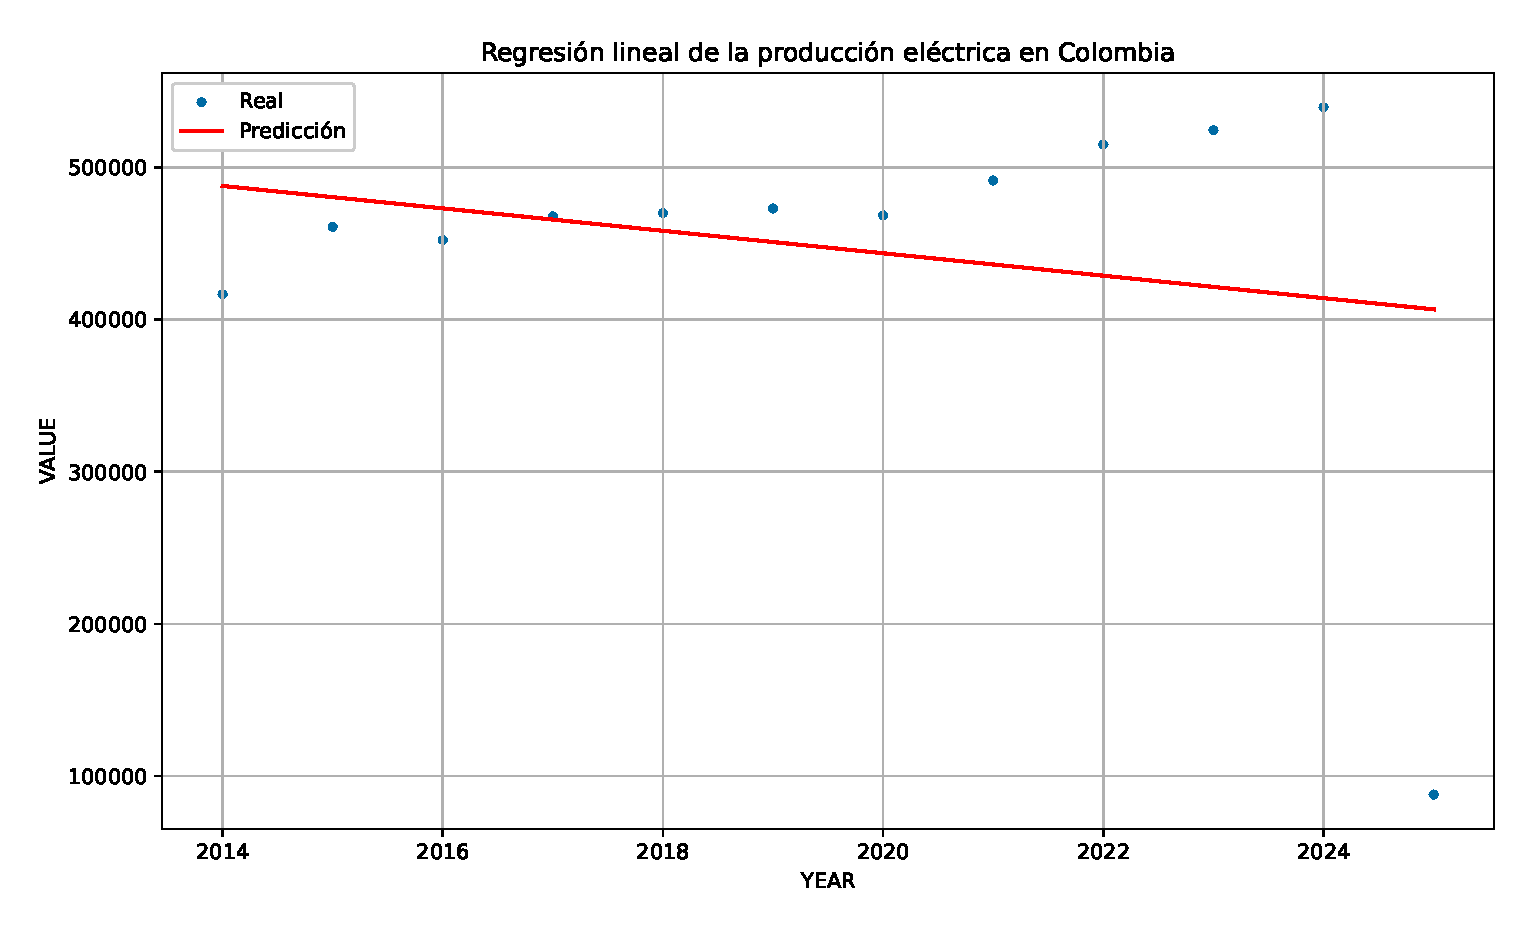
\includegraphics[width=0.7\linewidth]{fig_18}
	\caption{Regresión lineal de la producción eléctrica en Colombia}
	\label{fig:fig18}
\end{figure}


\subsection{An\'alisis de datos con aprendizaje no supervisado}

\subsubsection{Importaci\'on de librer\'ias y carga del archivo de trabajo}

\begin{minted}[]{python}
	# import library
	import pandas as pd
	import numpy as np
	from sklearn.linear_model import LinearRegression
	import matplotlib.pyplot as plt
	import seaborn as sns
	import os
	
	# set default directory
	os.chdir('/home/lbertel/code/talento_tech/content')
	
	# set style matplotlib
	plt.style.use('tableau-colorblind10')
	
	# load data
	colombia_df = pd.read_csv('data/processed/colombia_data.csv')
	colombia_df.head(10)
\end{minted}

{\tt
	\begin{tabular}{lllll}
		& YEAR & MONTH & PRODUCT                    & VALUE    \\
		0   & 2014 & 1     & Hydro                      & 3903.977 \\
		1   & 2014 & 1     & Wind                       & 5.648    \\
		2   & 2014 & 1     & Solar                      & 1.065    \\
		3   & 2014 & 1     & Coal                       & 521.938  \\
		4   & 2014 & 1     & Oil                        & 139.219  \\
		5   & 2014 & 1     & Natural gas                & 1031.146 \\
		6   & 2014 & 1     & Combustible renewables     & 99.721   \\
		7   & 2014 & 1     & Net electricity production & 5702.714 \\
		8   & 2014 & 1     & Electricity supplied       & 5555.847 \\
		9   & 2014 & 1     & Distribution losses        & 536.164 
	\end{tabular}
}

\subsubsection{Clustering de años según patrón energético (PCA + KMeans)}

\begin{minted}[]{python}
df_pivot = colombia_df.pivot_table(index='YEAR', columns='PRODUCT', values='VALUE', aggfunc='sum').fillna(0)

# 2. data scaling
scaler = StandardScaler()
data_scaled = scaler.fit_transform(df_pivot)

# 3. Reducing dimensions with PCA
pca = PCA(n_components=2)
pca_result = pca.fit_transform(data_scaled)

# 4. Group by with KMeans
kmeans = KMeans(n_clusters=3, random_state=42)
clusters = kmeans.fit_predict(pca_result)

# 5. show result
plt.figure(figsize=(10, 6))
sns.scatterplot(x=pca_result[:, 0], y=pca_result[:, 1], hue=clusters, palette='Set2', s=100)

# Añadir etiquetas de años
for i, year in enumerate(df_pivot.index):
plt.text(pca_result[i, 0]+0.02, pca_result[i, 1]+0.02, str(year), fontsize=9)

plt.title('Clustering de años según patrón energético (PCA + KMeans)')
plt.xlabel('YEAR')
plt.ylabel('VALUE')
plt.grid(True)
plt.tight_layout()
plt.show()
\end{minted}

\begin{figure}[t]
	\centering
	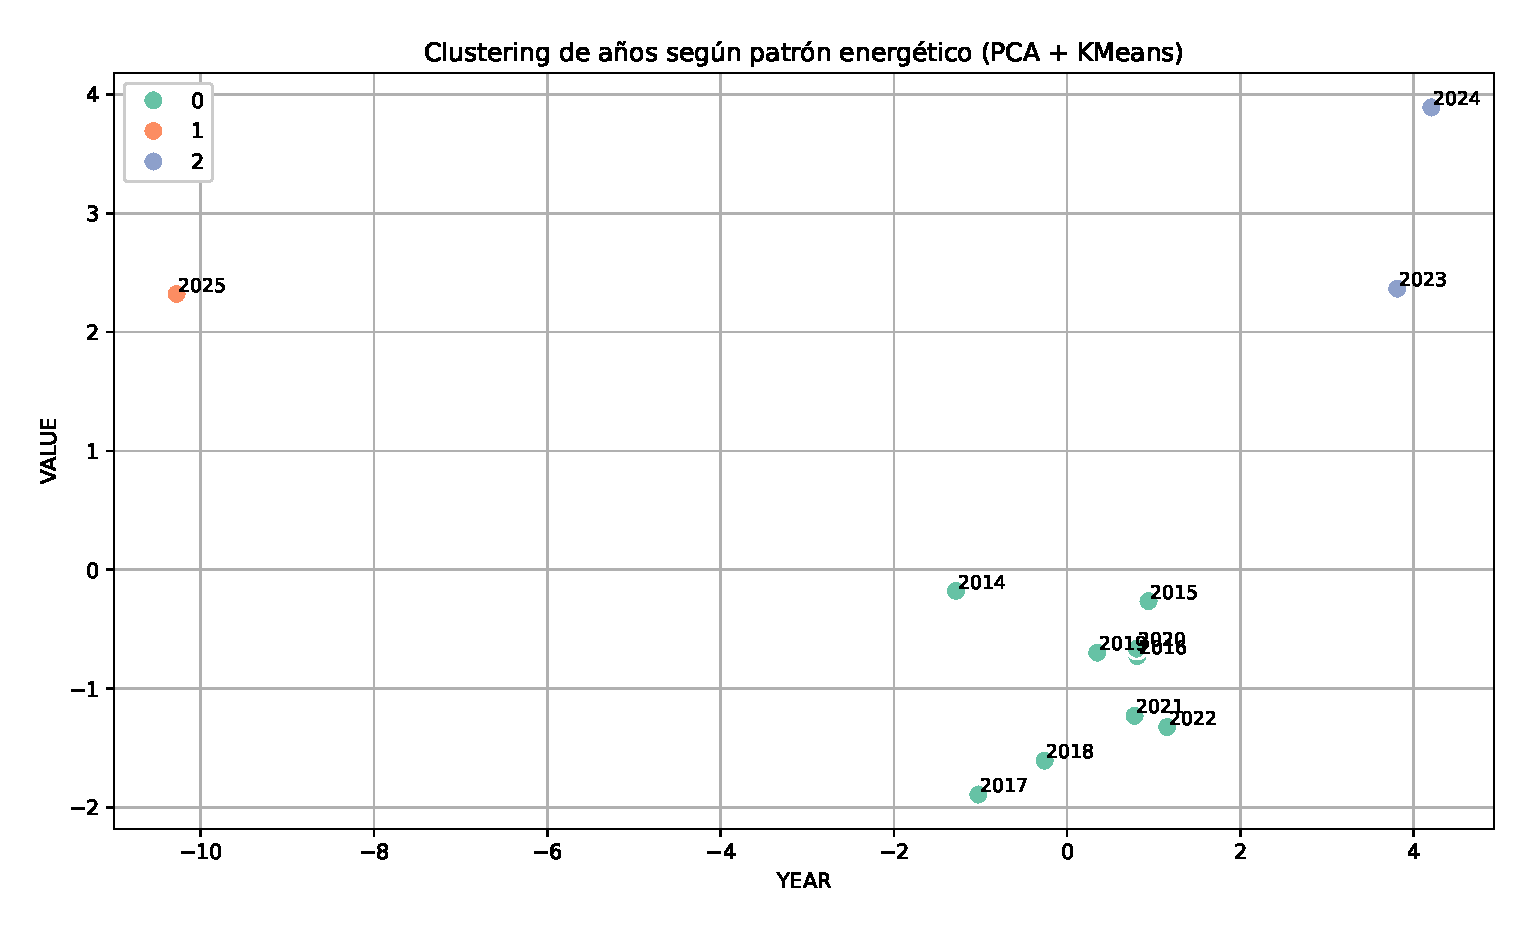
\includegraphics[width=0.9\linewidth]{fig_19}
	\caption{Clustering de años según patrón energético (PCA + KMeans)}
	\label{fig:fig19}
\end{figure}


\section{Conclusiones}

\begin{itemize}
	\item La generación hidroeléctrica domina ampliamente entre las fuentes renovables.
	\item Las fuentes como solar y eólica aún representan un porcentaje muy bajo, aunque con potencial de crecimiento.
	\item La energía basada en fósiles también tiene un peso relevante, especialmente el gas natural.
	\item Se observa un crecimiento sostenido de la producción entre 2014 y 2018.
	\item El análisis completo de 2019 a 2025 permitirá ver el impacto de políticas o proyectos recientes.
\end{itemize}

% Bibliografía --------------------------------------------------------
\bibliographystyle{apalike}
\bibliography{suministros_eficientes.bib}


%\addcontentsline{toc}{chapter}{Bibliografía} % agregar al Indice
%\begin{thebibliography}{99}
%\bibitem{Hahn} Hahn, J.``\fnte{LaTeX} $\,$ for eveyone''. Prentice Hall,
%New Jersey, 1993.
%\end{thebibliography}
\end{document}